\chapter{Method B: independent information extraction}
\chaptermark{Independent information extraction}
\label{chap:independent}
\graphicspath{{./chapters/4-independent/figs/}}

%Abstract-------------------------------------------------------------------------------------------------------------
%In this chapter we propose a symbol spotting technique in graphical documents. Graphs are used to represent the documents and an error tolerant (sub)graph matching technique is used to detect the symbols in them. We propose a graph serialization to reduce the usual computational complexity of graph matching. Serialization of graphs is performed by computing acyclic graph paths between each pair of connected nodes. Graph paths are one dimensional structures of graphs, handling which is less expensive in terms of computation. At the same time they enable robust localization even in the presence of noise and distortion. Indexing in large graph databases involves a computational burden as well. We utilize a graph factorization approach to tackle this problem. Factorization is intended to create a unified indexed structure over the database of graphical documents. Once graph paths are extracted, the entire database of graphical documents is indexed in hash tables by locality sensitive hashing (LSH) of shape descriptors of the paths. The hashing data structure aims to execute an approximate $k$-NN search in a sub-linear time. We have performed detailed experiments with various datasets of line drawings and the results demonstrate the effectiveness and efficiency of our technique.
%----------------------------------------------------------------------------------------------------------------------

In this chapter we propose an independent extraction of each element contained by comic book images.
This content retrieval approach tries to fill the weaknesses of the sequential approach presented in the previous chapter.
New approaches for extracting panels, text, balloons and comic characters are presented successively but they can be used in any order as they are completely independent for each other.
New domain knowledge are embedded in the low level processing to process each image in and autonomous way with a similar performance.


\section{Introduction}
\label{sec:in:intro}

\modif{TODO or REMOVE}

\section{Panel extraction}
\label{sec:in:panel_extraction}

The previous clustering-based method presented in Section~\ref{sec:se:panel_and_text} is particularly useful for simultaneous extractions, as illustrated panel and text while removing noise region at the same time.
Nevertheless, the panel extraction can be improved if we focus on panel elements only.
We propose to use a second characteristic of panels which is their topological relations with other elements in the image.
Figure~\ref{fig:se:cc_bounding_box} shows that outermost or external contours actually corresponds to panels.
We base this method on this criterion, considering the panels to be the outermost contours.
This is especially true for general comics using gutter (white space) between panels.
Making the outermost contour as panel can be seen as a binary classification method deriving from a more generic concept.
The general concept would attribute a confidence value to each contour in the image, inversely promotional to their percentage of inclusion in other contours.
Non included contour (outermost) would have the maximum confidence and fully included ones the lowest confidence in being a panel.

% We propose to combine the advantages of the already published panel extraction methods~\cite{Arai11,Rigaud2012LNCS} and partially solve their weaknesses using the expert system model.
% that we present section~\ref{sec:expert_system}.
% They are connected component based methods that are reliable for comics with disconnected panels (separated by gutters).
% no gutter between the panels (they are separated by a single black line).
% Line-based decomposition methods are the efficient methods for line separated comics~\cite{Li2013Unsupervised} (no gutter).
% A generic method that works best with both styles is not obvious.
% We combine~\cite{Arai11,Rigaud2012LNCS} to introduce a new method, especially suitable for general comics using gutter (white space) between panels.

Panel contours (border line) are usually dark and similar for all the panels of a comics page.
Sometimes panel contours are implicit as shown Figure~\ref{fig:in:se:panel_img} (considered as a difficult case).
In this case, the reader distinguishes them by comparing the difference of colour between the panel content and the page background.
We use a global binary segmentation method (Section~\ref{sub:ap:bi_threshold}) to separate the page background (expected to be clear) from its content (dark elements such as panel border lines), considered as foreground here (Figure~\ref{fig:se:panel_binary}).
An binary inversion should be performed when the image background is darker that the content of the panels.
We do not use a local segmentation approach here because it has higher chances to split the panel border and over-segment its content.

Then, a connected-component labelling algorithm (Section~\ref{sec:ap:connected_component_labelling}) is used to extract outermost contours from the binary image, (Figure~\ref{fig:in:panel_outermost_contours}).
Note, we filter out contours below a minimum area relative to the image size $minAreaFactor$ in order to avoid considering isolated elements (e.g text, logo, page number) as panel in a later stage (Figure~\ref{fig:in:panel_big_contours})

Finally, the convex hull or the bounding box of the panel contours can be computed in order to recover from discontinuous contour detection (Figure~\ref{fig:in:panel_big_contour_hull} and~\ref{fig:in:panels_detection_boxes}).
In this example, some of the panel borders have low contrast compared to the page background which makes difficult their extraction.
Such issue can be post processed using line detection and layout analysis.

% Here we improve the binary image segmentation using adaptive thresholding method to overcome digitization variations.
% Adaptive thresholding consist in deciding if a pixel at position $(x,y)$ belongs to the foreground or background according to the mean value of its neighbourhood pixels in a window of size $blockSize * blockSize$.
% % r each pixel position $T(x,y)$ is a mean of the $blockSize * blockSize$ neighbourhood of point of coordinates $x,y$.
% The $blockSize$ is an odd value related to the image size as defined by equation~\ref{eq:panel_blockSize}.
% Note, we add one to the $blockSize$ value if is not odd in order to make sure the point $(x,y)$ is always at the centre the window.

% \begin{equation}
% \label{eq:panel_blockSize}
% 	blockSize = \frac{I_{width} + I_{height}}{2} * blockSizeFactor
% \end{equation}
% where $blockSizeFactor$ corresponds to a constant discussed section~\ref{sec:se:experimental_results}. 


%%%%%%%%%%%%%%%%%%%%%%%%%%%%%%%%%%%%%%%%%%%%%%%%%%%
 % \begin{figure}[!ht]  %trim=l b r t  width=0.5\textwidth,
 %   \centering
 %  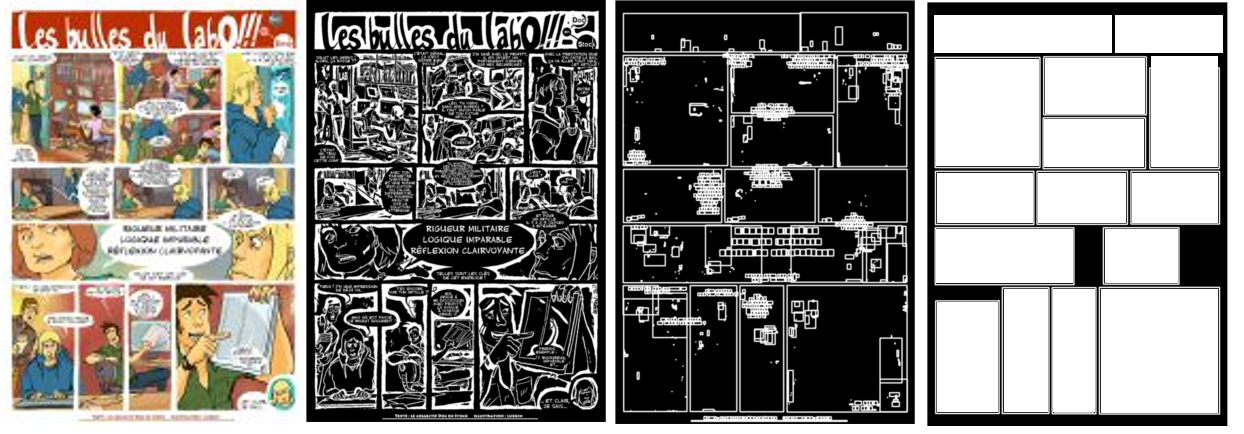
\includegraphics[width=1.0\textwidth]{panel_detection.png}
 %  \caption{Contour detection and filtering of panel.
 %  Original image, adaptive thresholding, contour bounding boxes and results mask of the outermost contours from left to right.}
 %  \label{fig:panel}
 % \end{figure}
%%%%%%%%%%%%%%%%%%%%%%%%%%%%%%%%%%%%%%%%%%%%%%%%%%%

%%%%%%%%%%%%%%%%%%%%%%%%%%%%%%%%%%%%%%%%%%%%%%%%%%%
\begin{figure}[!ht]	%trim=l b r t  width=0.5\textwidth, 
  \centering
	%\includegraphics[height=60mm]{figure/BUBBLEGOM_T01_P007_crop.jpg}
	%\includegraphics[trim= 0mm 0mm 0mm 0mm]{figure/BUBBLEGOM_T01_P007.jpg}
	\subfloat[Original image]{\label{fig:in:se:panel_img}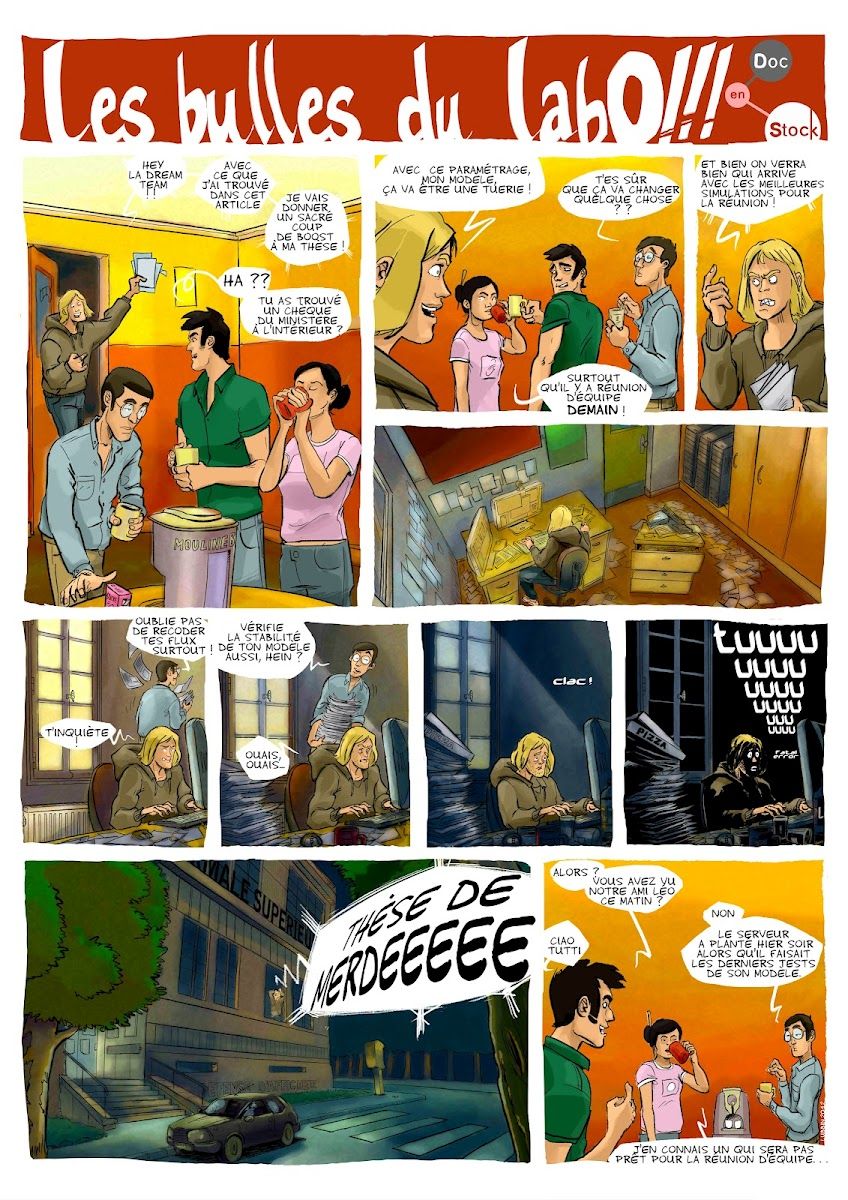
\includegraphics[trim= 0mm 0mm 0mm 0mm, clip, width=0.27\textwidth]{panel_img.jpg}}
	\hspace{1em}
	\subfloat[Binary segmentation]{\label{fig:se:panel_binary}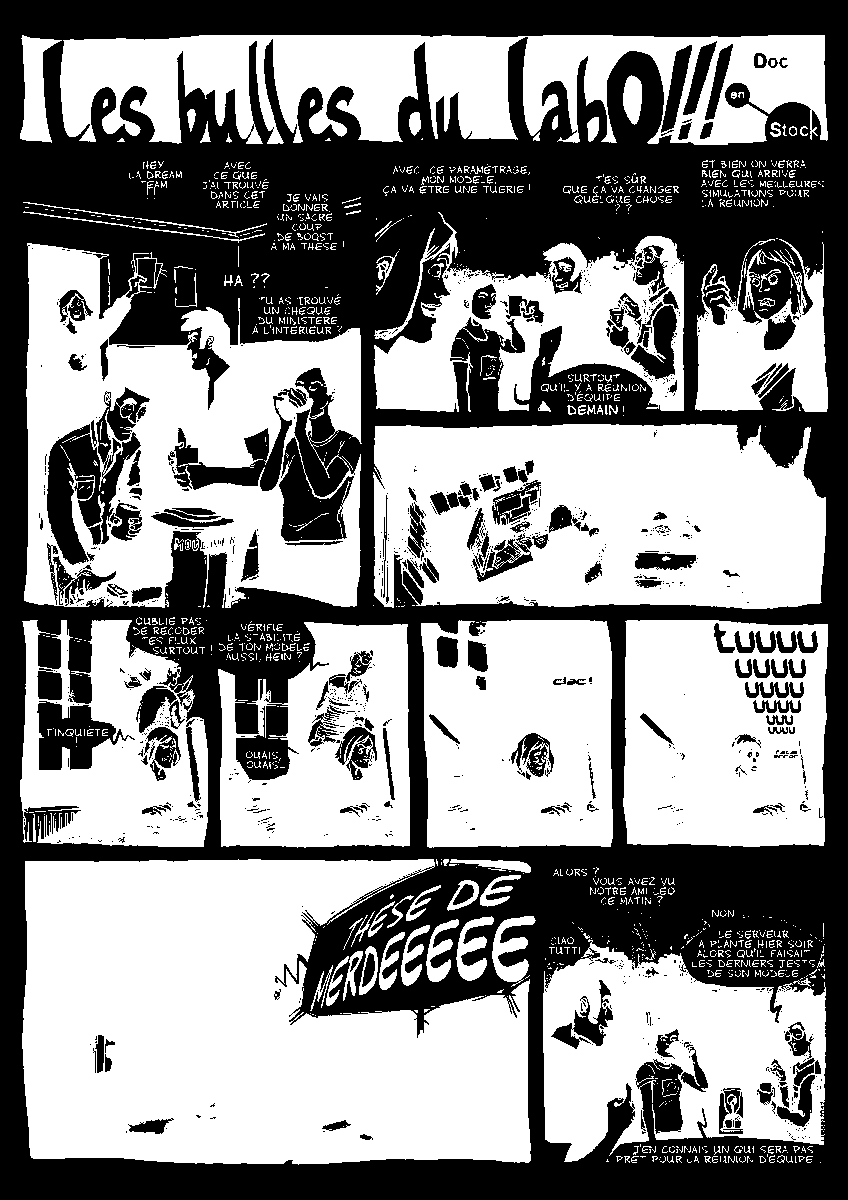
\includegraphics[trim= 0mm 0mm 0mm 0mm, clip, width=0.27\textwidth]{panel_binary.png}}
	\hspace{1em}
	\subfloat[Outermost contours]{\label{fig:in:panel_outermost_contours}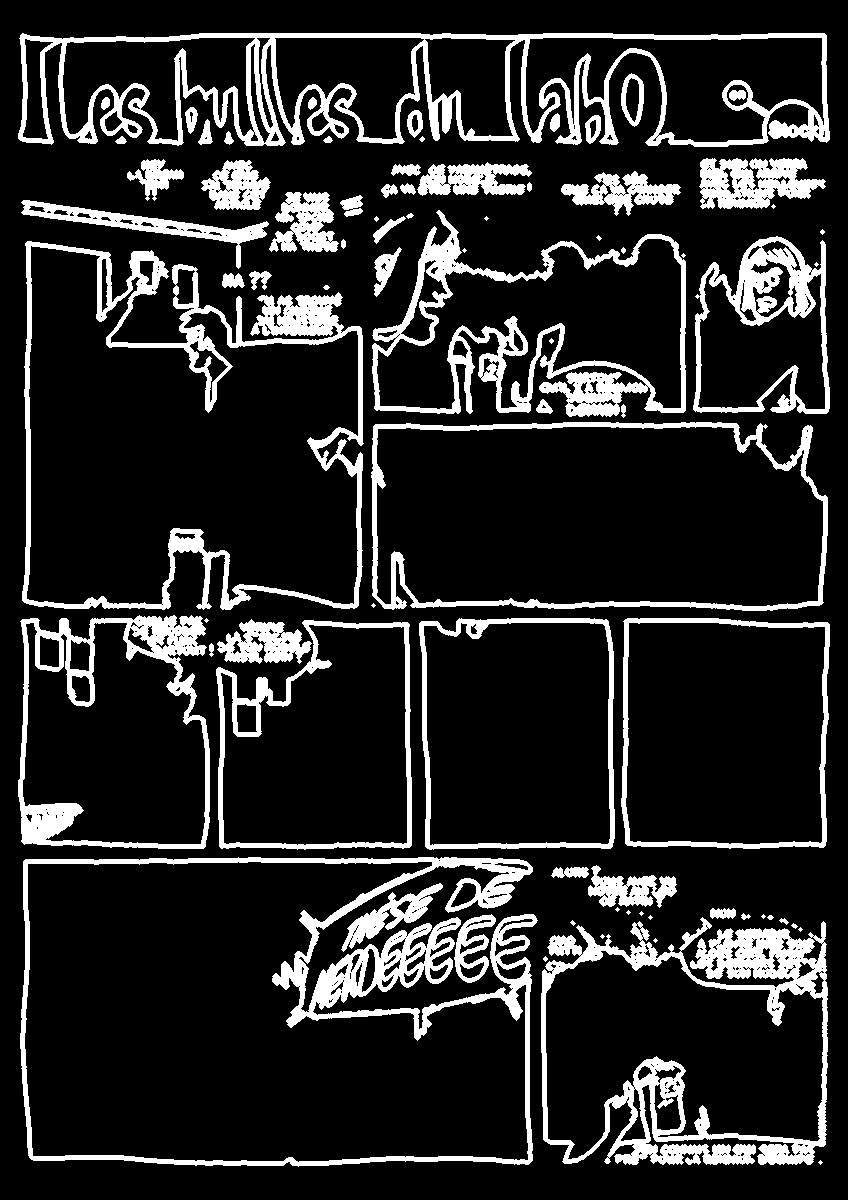
\includegraphics[trim= 0mm 0mm 0mm 0mm, clip, width=0.27\textwidth]{panel_all_contours.png}}
	\\
	\subfloat[Panel contours]{\label{fig:in:panel_big_contours}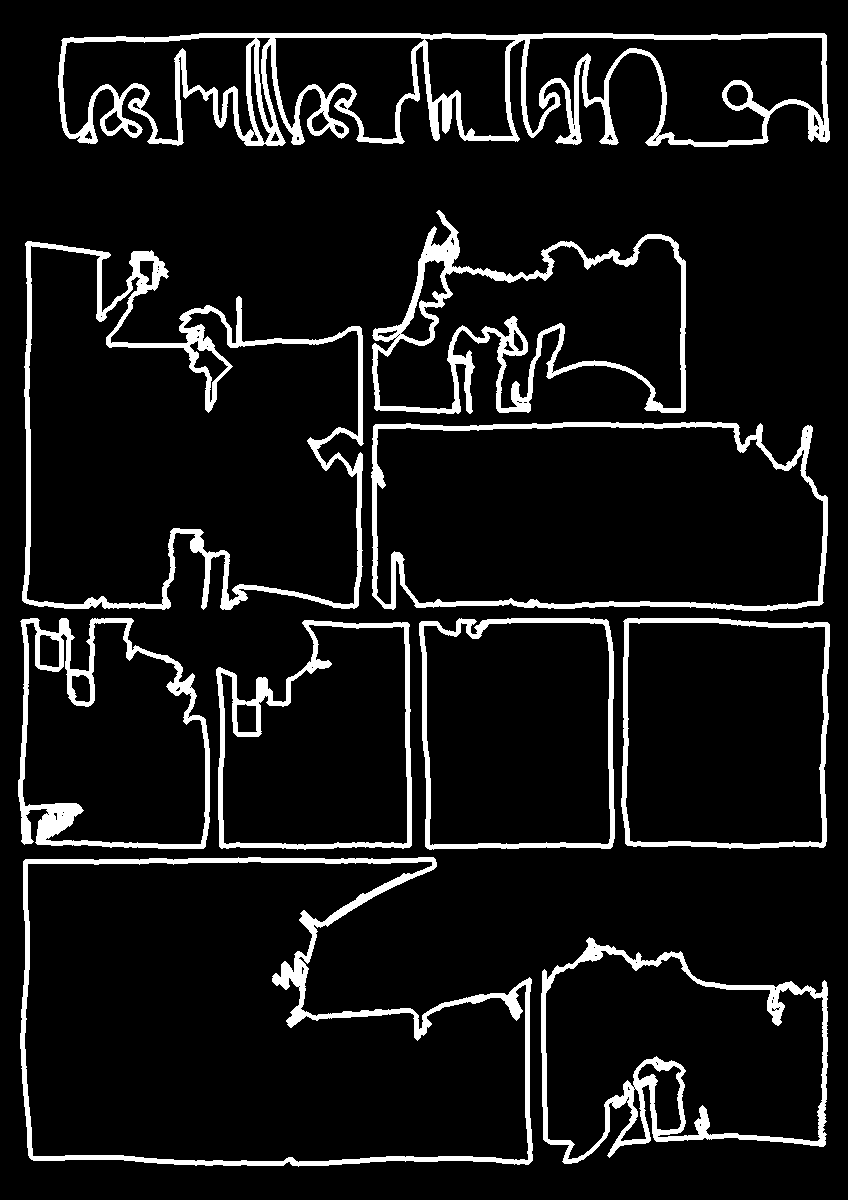
\includegraphics[trim= 0mm 0mm 0mm 0mm, clip, width=0.27\textwidth]{panel_big_contours.png}}	\hspace{1em}
	\subfloat[Panel contour hulls]{\label{fig:in:panel_big_contour_hull}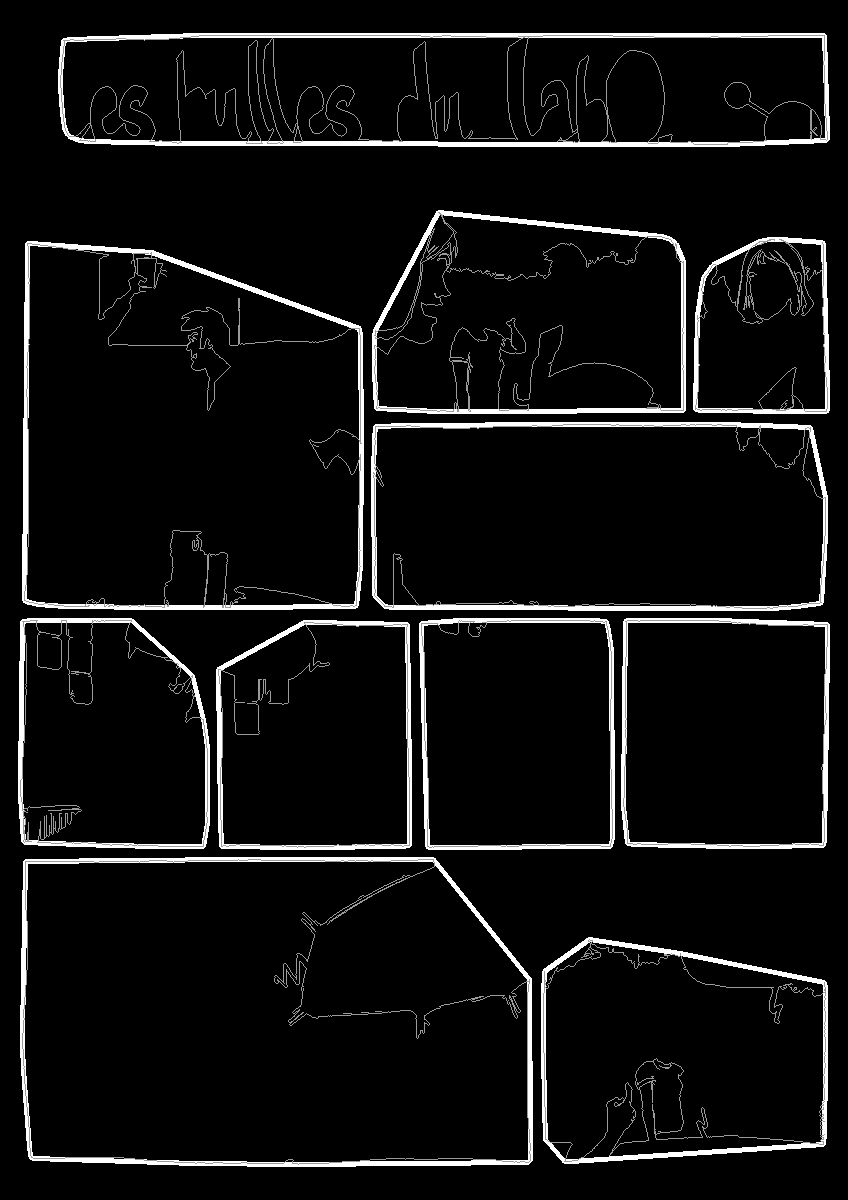
\includegraphics[trim= 0mm 0mm 0mm 0mm, clip, width=0.27\textwidth]{panel_big_contour_hull.png}}
	  \hspace{1em}
	\subfloat[Panel contour bounding boxes]{\label{fig:in:panels_detection_boxes}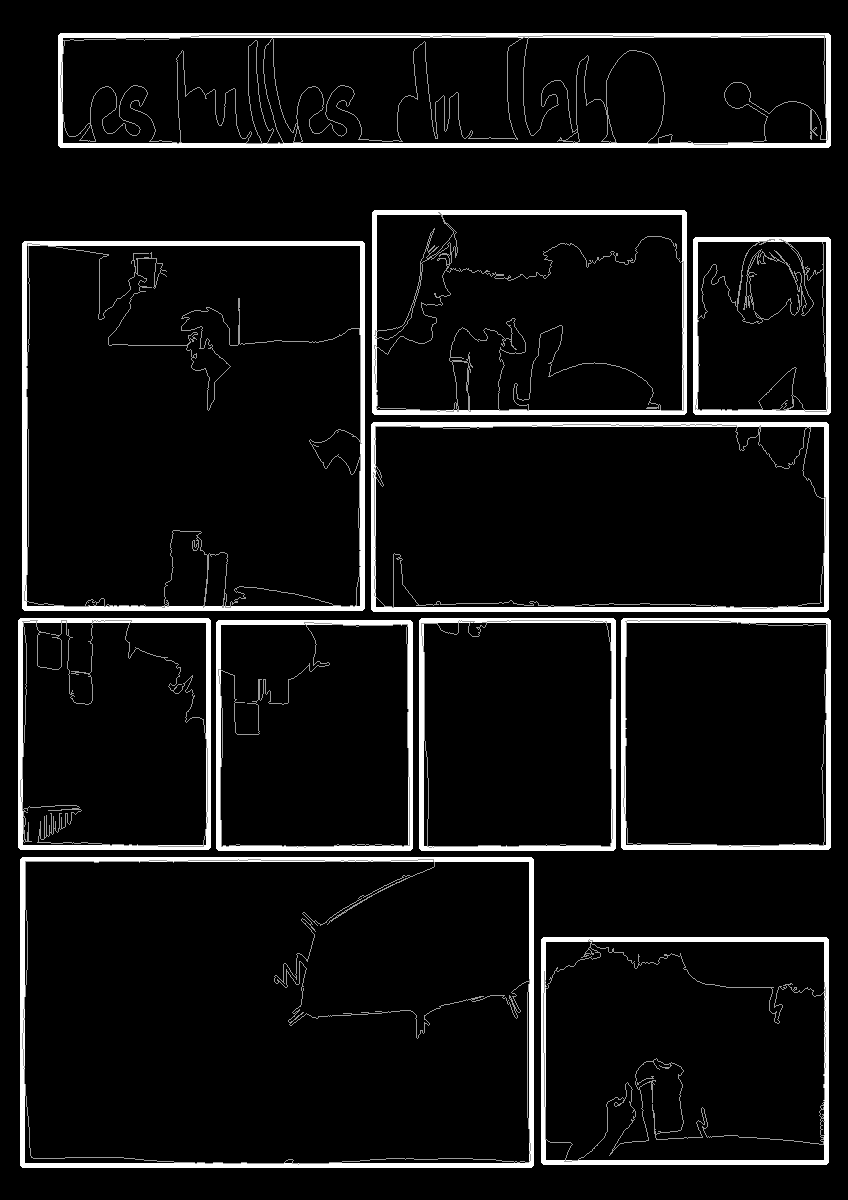
\includegraphics[trim= 0mm 0mm 0mm 0mm, clip, width=0.27\textwidth]{panels_detection_boxes.png}}
	  \caption[Independent panel extraction process]{Panel extraction process. Image credits:~\cite{Lubbin12}.}
	  \label{fig:in:panel_detection_process}
\end{figure}
%%%%%%%%%%%%%%%%%%%%%%%%%%%%%%%%%%%%%%%%%%%%%%%%%%%


\section{Text localisation and recognition} % (fold)
\label{sec:in:text_localisation_and_recognition}

In this section we present a method for automatic text localization in scanned comic books, an essential step towards an automatic comics understanding.
Our first intention is to localize multi-oriented text regions, independently from script and language, and separate them from the graphical content (text/graphic separation).
In document analysis systems, text recognition quality often relies on text localization.
This is particularly the case for comics which have a complex background.
We present how to take advantage of Optical Character Recognition systems (OCR) in order to improve text localisation.

\subsection{Introduction} % (fold)
\label{sub:in:text_introduction}

In comic book documents, text is mixed with graphical content which produces a lot false detections if we submit the whole image directly to an OCR system, usually coupled with a layer analysis pre-processing to avoid trying to recognize text in graphical region (e.g images, tables and formulas).
The mixture of typewritten, handwritten-like and handwritten text makes the task particularly difficult for comics.
Moreover, text presents a lot of variations (e.g. stroke, orientation, colour, size) that can cause many issues at both the localization and recognition levels.
Text localization aims to provide text-only (or graphics-free) images to a text recognition system in order to improve its accuracy and reduce computing time.
Knowing the positions of other elements in the image is a good clue for predicting text position because they are related to speech balloons (e.g. dialogue, thought), characters (e.g. graphic sound, illustration), panels (e.g. captions) or the page itself (e.g. page number, title, author name), this approach is discussed \ch{chap:knowledge}.

Few works concern text extraction in comics analysis literature (Section~\ref{sec:sota:text}) and most of them rely on speech balloon regions which make them dependent on other processing quality.
Here we want to avoid such dependency between processes.
From our knowledge, only Li~\cite{Li2013Unsupervised} proposed an independent and unsupervised speech text localization.
It is a two step analysis that first generates text lines using ``a set of very rigorous rules'' to test each pair of connected component and decide if they are candidate text regions or not.
From the first-round generated text lines, the method automatically learns a font set which is propagated to all text lines in the second-round and filters out non font-matched candidate regions.
The font set is generated from the distribution of heights and widths of the connected components that compose the candidate text line (composed by multi-segment characters).
The method is promising but there are nine rules in total that must be met to achieve text line extraction with several heuristics that are not discussed.
The experiments have been performed on 1000 images from 10 countries (balanced) but they are unfortunately not publicly available to assess their diversity and the genericity of this approach. 

The genericity is always a challenge for document image analysis, especially because this field of research is highly application dependent (Section~\ref{sec:document_image_analysis}).
Moreover, comic book images differ from classical documents in that they comprise complex backgrounds of a graphical nature.
They belong to the class of non-structured documents meaning there is no regular structure present for the prediction of text locations and no layout analysis method applicable if we consider all the diversity of comics.
Comics being unstructured graphical documents, combine the difficulties of both domains, making the task of text localization especially challenging.
To solve the particular problems which are provoked by the combination of complex background and unstructured documents, we propose a new text localization method.
% We improve the initial segmentation step to cope with complex backgrounds.
% Furthermore, we adapt the text line extraction method to cope with unstructured documents.

The contributions come at different levels. 
First, an adapted binary segmentation method is presented followed by a text/graphic separation algorithm based on the local contrast and neighbourhood similarities and finally, text recognition is used to verify the presence of textual information in the result.

% \subsection{Text localization} % (fold)
% \label{sub:te:text_localization}


\subsection{Bi-level segmentation}
\label{sec:in:segmentation}
Segmentation is a crucial step in many text localization methods.
Comic speech text is made of strokes, generally black on white, that we would like to isolate from the rest of the image content (background).
A perfect text segmentation would result to individual text letters represented by single connected components (Section~\ref{sec:ap:connected_component_labelling}).
The complex background of comic documents complicates this step.
Separating text from other elements in once is quite hard since we have no information about its position (independent approach) and it is similar to many other stroke in the image.
Therefore, we propose first to separate bright from dark regions and then classify text and non text regions using size and alignment properties only.
This approach is unsupervised and do not requires any training step.
Bright/dark region separation can be done using a bi-level segmentation algorithm.
Several approaches exist and their performance relies on the input data distribution.
If the input data are composed by only black or white pixels any method will do the work be it is rarely the case.
The best input would be a highly contrasted image where the feature of interest are concentrated in one of the extrema.
As we do not use the colour information, we convert the 3 channel colour image (RGB) into a single channel grey image.
There are several manners to create a grey-scale image from a colour image.
The first approach is to combine each pixel value from each colour channel with different weighting coefficients corresponding to the measured intensity perception of typical trichromat humans\footnote{\url{http://en.wikipedia.org/wiki/Grayscale}}, in order to produce a single value per pixel.
Another approach is to use only one channel but as the text we are interested in is not in red, green or blue (RGB colour space) it is irrelevant in our case.
Nevertheless, RGB colour space can easily be converted to a different colour space such as HSV or HSL that encodes colours as Hue, Saturation, Value or Luminance.
The luminance channel is particularly appropriate for bright and dark region separation~\cite{Ho2012}.

Even if looking at the pixel from the luminance point of view is more appropriate for our purpose, we still need to determine the threshold value that will best divide the grey value distribution into two clusters (Figure~\ref{fig:in:greyscale_text_pixel_distribution}).


% 	%%%%%%%%%%%%%%%%%%%%%%%%%%%%%%%%%%%%%%%%%%%%%%%%%%%
	\begin{figure}[h!]	%trim=l b r t  width=0.5\textwidth,
	  \centering
		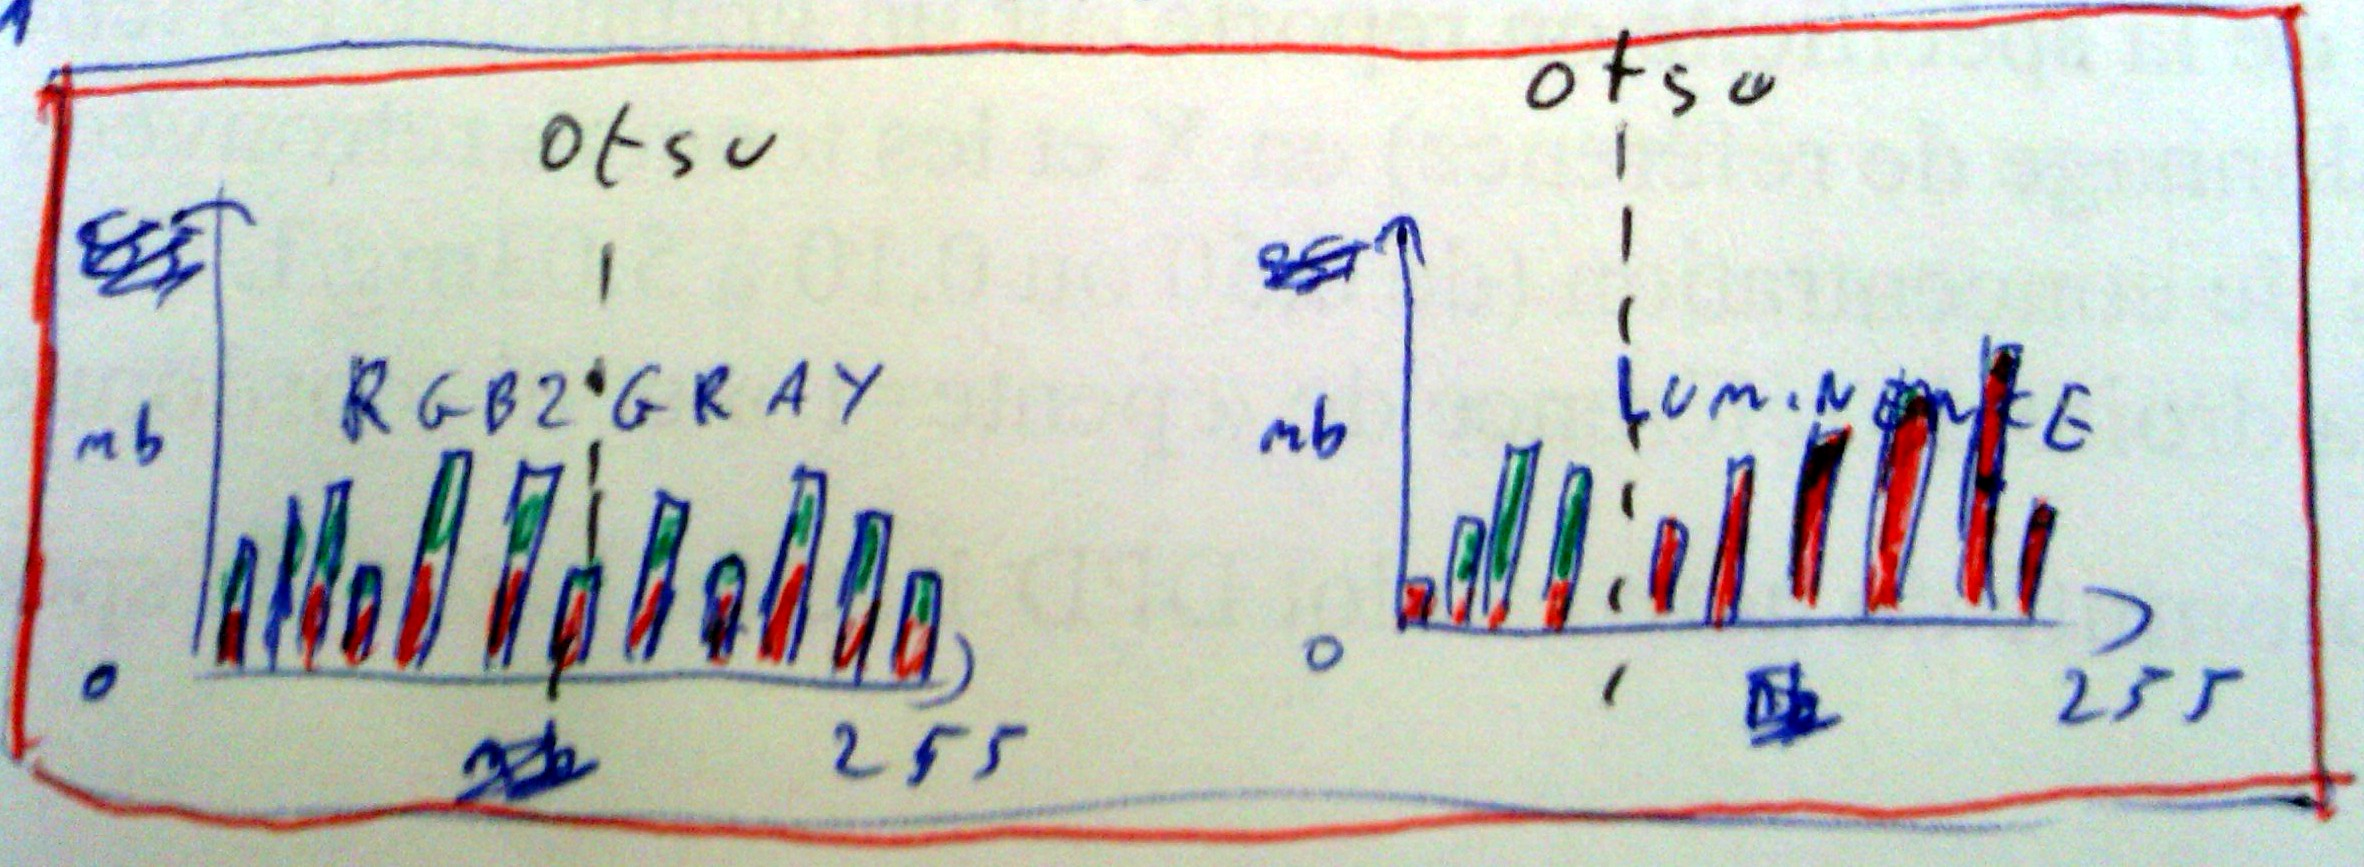
\includegraphics[trim= 0px 0px 0px 0px, clip, width=0.75\textwidth]{threshold_selection_methods.jpg}
		\caption[Grey scale image pixel value distribution for text and non text region]{Grey scale image pixel value distribution and text repartition. The percentage of pixel belonging to text regions are in green, others in red \modif{TODO: update figure}.}
		\label{fig:in:greyscale_text_pixel_distribution}
	\end{figure}
% 	%%%%%%%%%%%%%%%%%%%%%%%%%%%%%%%%%%%%%%%%%%%%%%%%%%%

Fixing a threshold value like Arai's method~\cite{Arai11} works only for few comics type with a same text background intensity (Figure~\ref{fig:in:threshold_selection_methods}).
This phenomenon is intrinsic to the nature of comics, as due to the design process they contain textured areas and loosely connected strokes that give rise to merged components at different thresholds.
This is intensified by the digitization and image compression process that adds further noise to the page (Section~\ref{sec:document_image_analysis}).
Instead of using a fixed threshold, we use the well known Otsu's threshold selection method that have been extensively use since decades for this purpose (Section~\ref{sub:ap:bi_threshold}).
Otsu's threshold is computed for each image and applied to the whole image assuming that the image have not been degraded locally.
In case of such local degradation (e.g. holes, crossed text, partial erasure, highlighting, tearing paper, stain), a local threshold selection method should be used (Section~\ref{sub:ap:bi_threshold}).


% 	%%%%%%%%%%%%%%%%%%%%%%%%%%%%%%%%%%%%%%%%%%%%%%%%%%%
	\begin{figure}[h!]	%trim=l b r t  width=0.5\textwidth,
	  \centering
		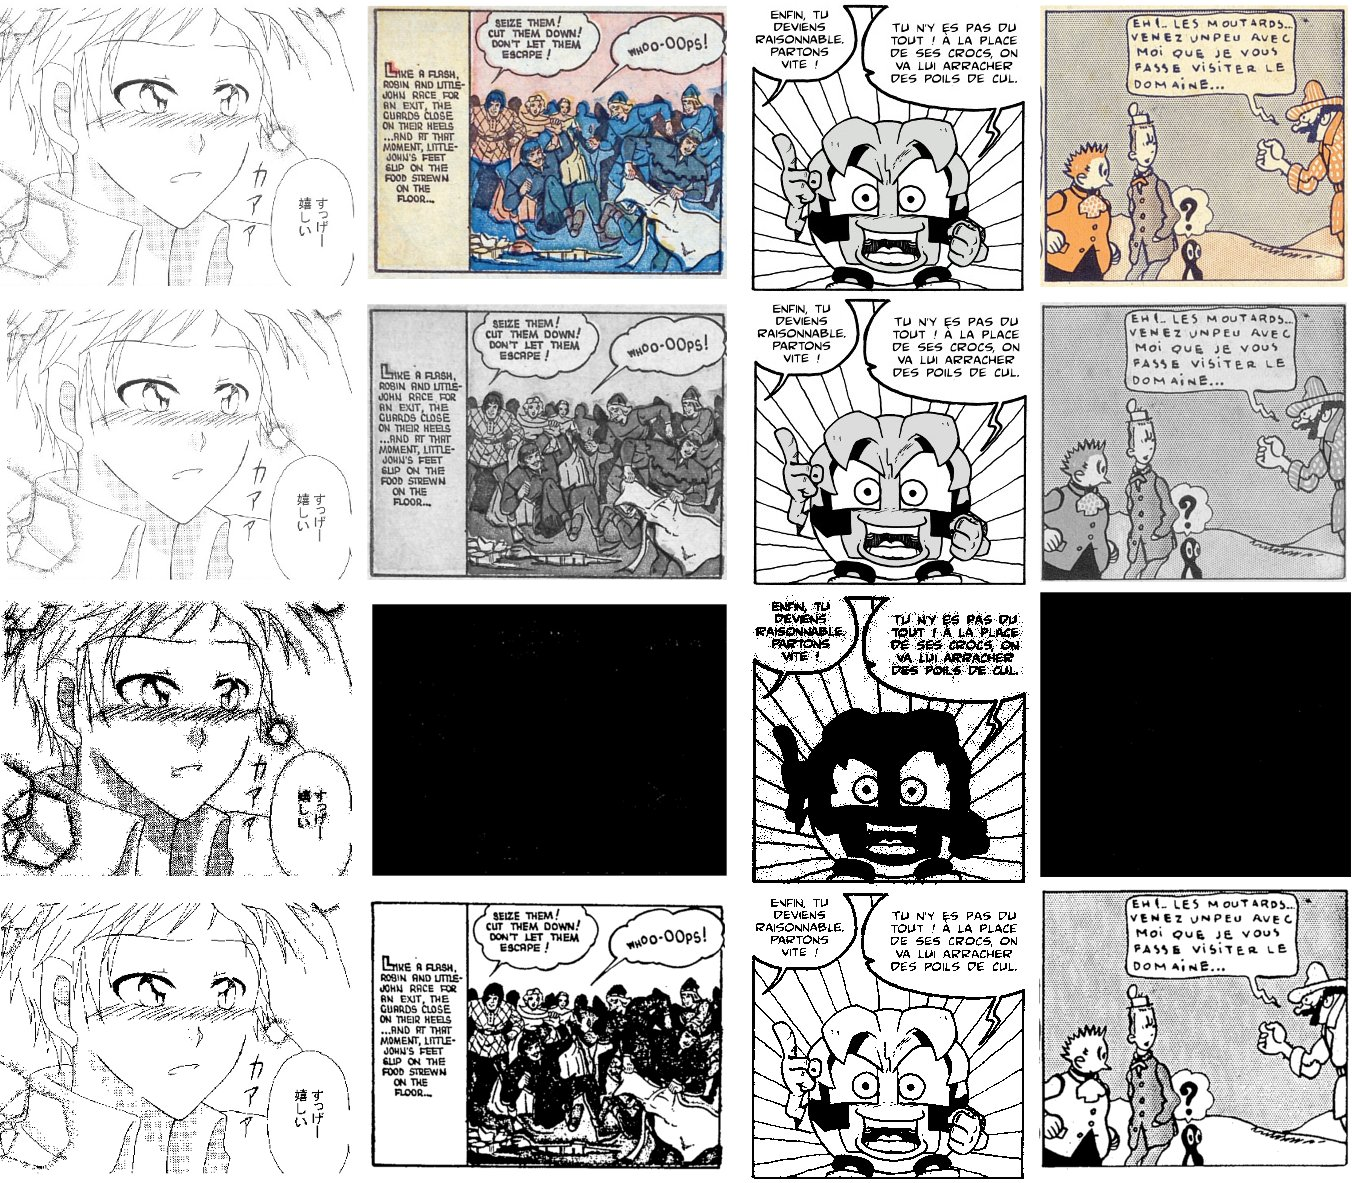
\includegraphics[trim= 0px 0px 0px 0px, clip, width=0.95\textwidth]{threshold_selection.jpg}
		\caption[Different threshold selection applied on a grey-scale image]{Different threshold selection methods applied on the luminance channel of several comics types. First row shows the original image of a selection of comic book parts. Second row shows the corresponding luminance channel of HSL colour space in a 8 bits grey-scale image. The third row represents the bi-level segmentation of the grey-scale image with a fixed threshold at 250 (as Arai~\cite{Arai11}) and fourth row shows the corresponding results using the automatic Otsu's threshold selection method.}
		\label{fig:in:threshold_selection_methods}
	\end{figure}
% 	%%%%%%%%%%%%%%%%%%%%%%%%%%%%%%%%%%%%%%%%%%%%%%%%%%%




%Typical thresholding methods would fail to segment the text because text is drawn with the same style of strokes as many other graphical elements in the page \modif{TODO: delete + explain the interest of choosing a good threshold, refer the standard Otsu from SOTA, its interest and the importance of its input (gray image). Assuming that text is written in dark over bright background or vice versa, we don't need the colour information (assuming we don't want to extract coloured text with this method). The widely used RGB2GRAY conversion combine the colour channel to produce a grey image. As we don't need the colour information, we convert RGB to HSL ans use the luminance layer as input for Otsu auto threshold selection. (illustrate the differences between Otsu'method applied on RGB2GRAY, H, S and L.)}.

%Therefore, we propose to improve the Otsu's threshold selection method~\ref{sub:ap:bi_threshold}.
%For a single page we assume that the text background brightness is similar around all the characters of the same page. However, in our case, the optimal segmentation threshold differs for every single page of comics depending on the background colour of the text areas. The method is based on the observation that choosing the threshold too low, as well as choosing the threshold too high leads to an over segmentation of the connected components (CC) (Figure~\ref{fig:in:bin}).

	%%%%%%%%%%%%%%%%%%%%%%%%%%%%%%%%%%%%%%%%%%%%%%%%%%%
	% \begin{figure}[h!] %trim=l b r t
	%   \begin{center}$
	%     \begin{array}{cccc}
	%       \fbox{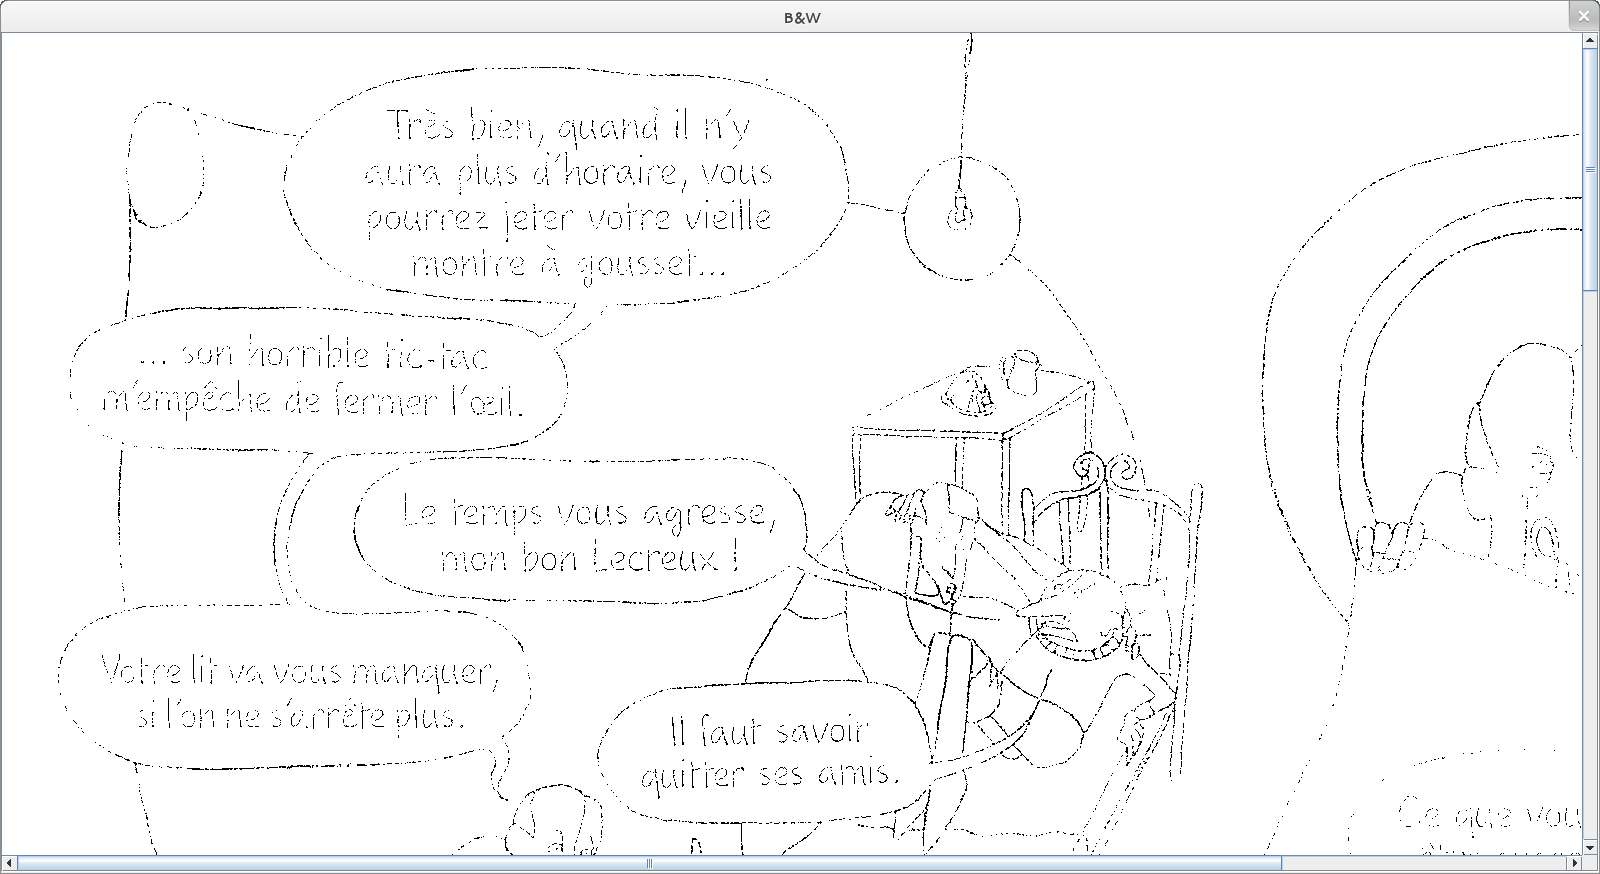
\includegraphics[trim= 597px 20px 500px 400px, clip, width=0.22\textwidth]{bin_50.png}} &
	%       \fbox{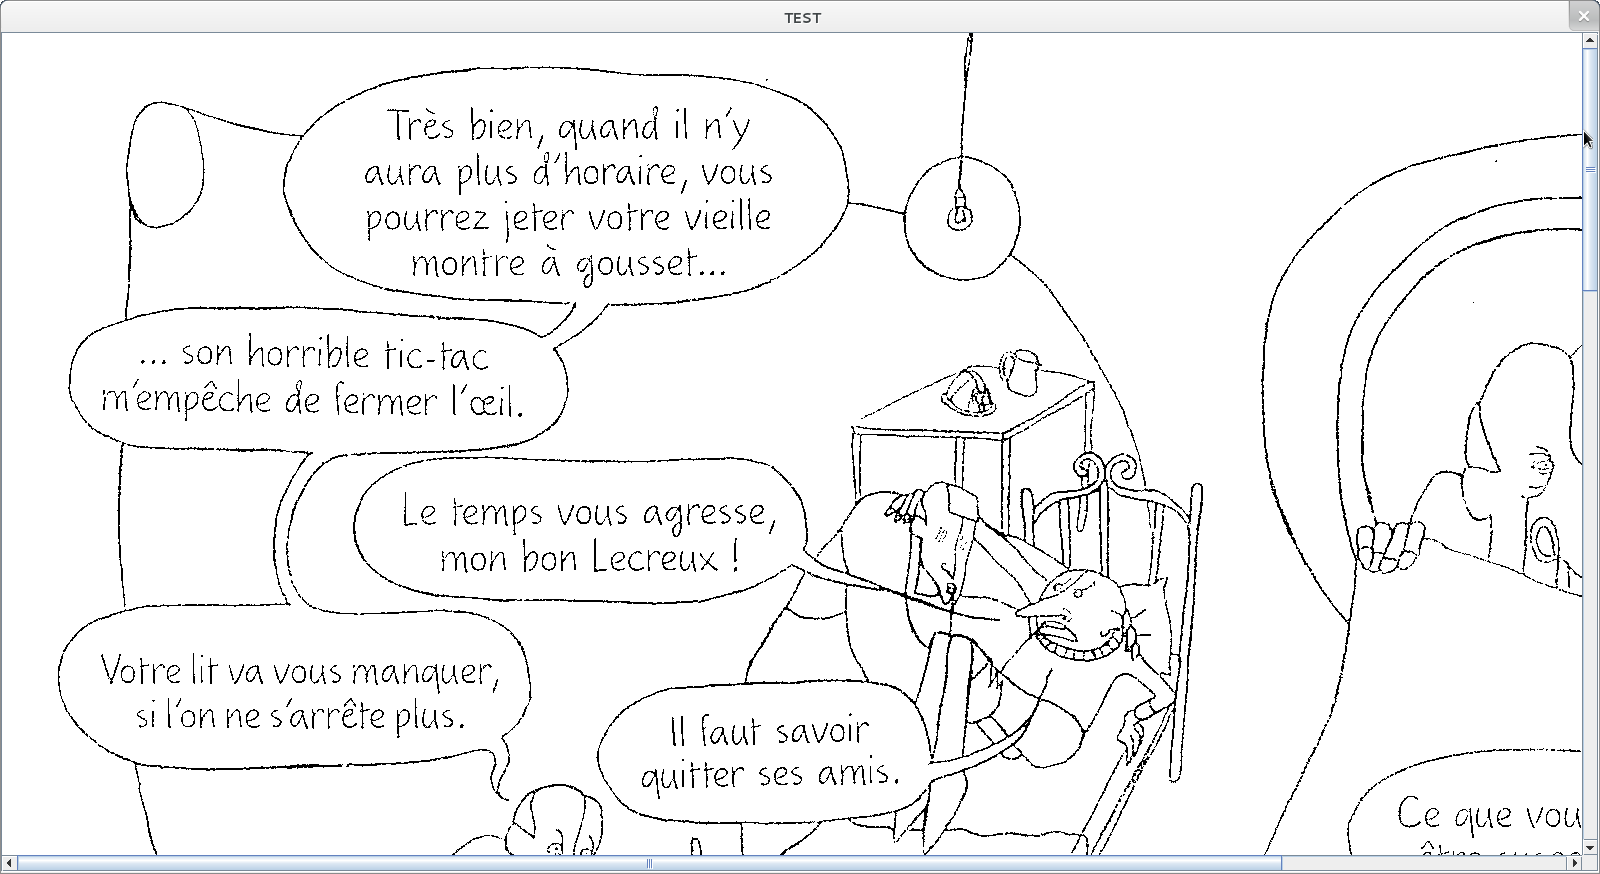
\includegraphics[trim= 597px 20px 500px 400px, clip, width=0.22\textwidth]{bin_80.png}}  \\
	%       \fbox{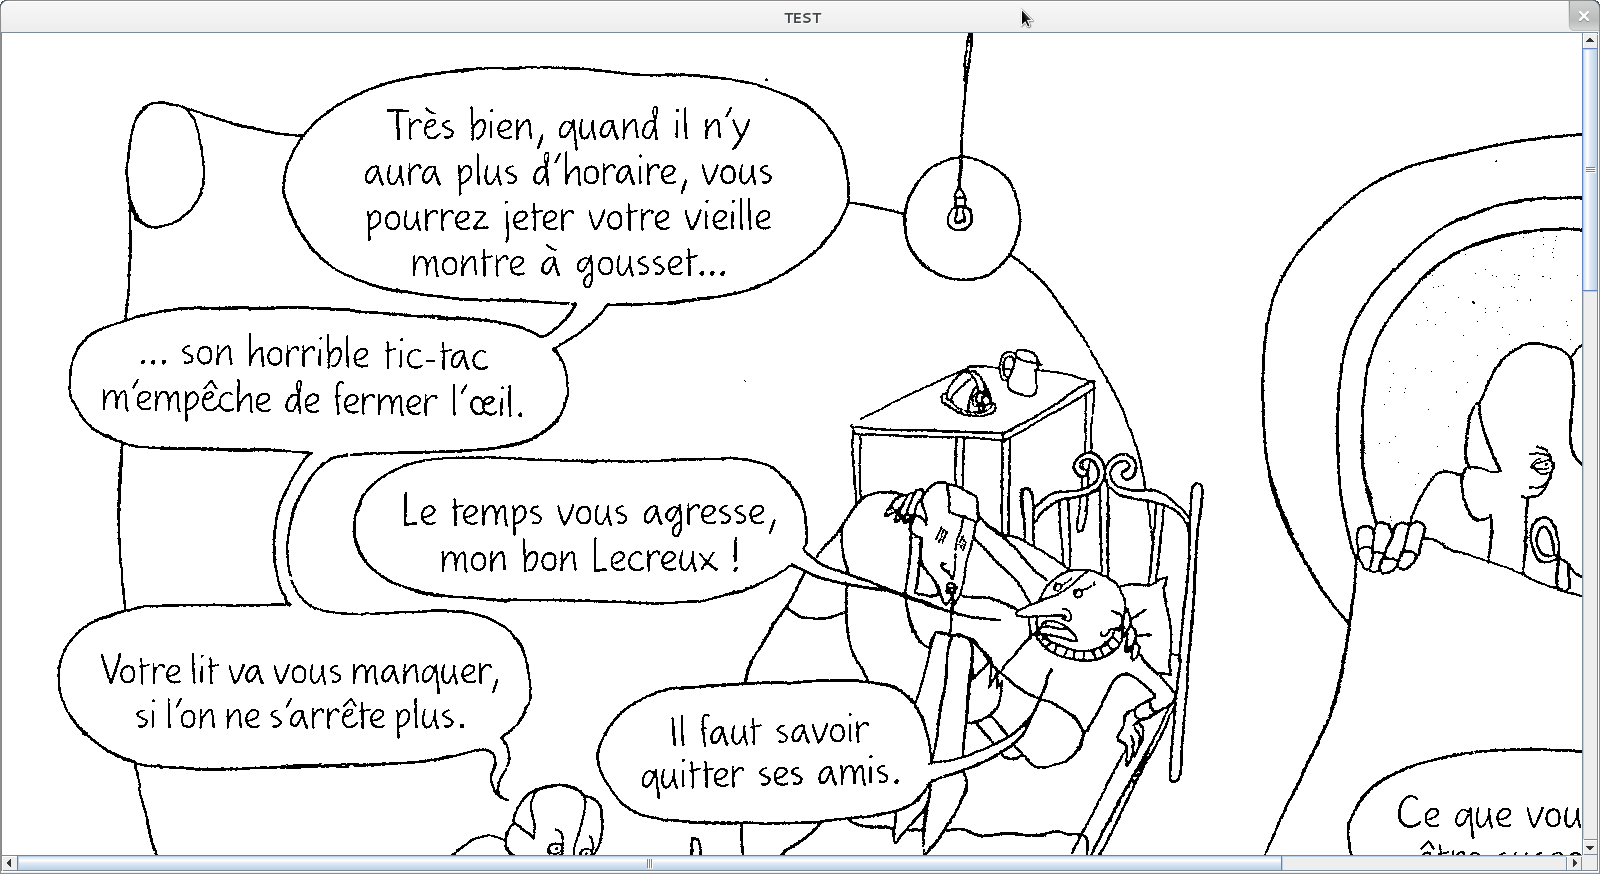
\includegraphics[trim= 597px 20px 500px 400px, clip, width=0.22\textwidth]{bin_120.png}} &
	%       \fbox{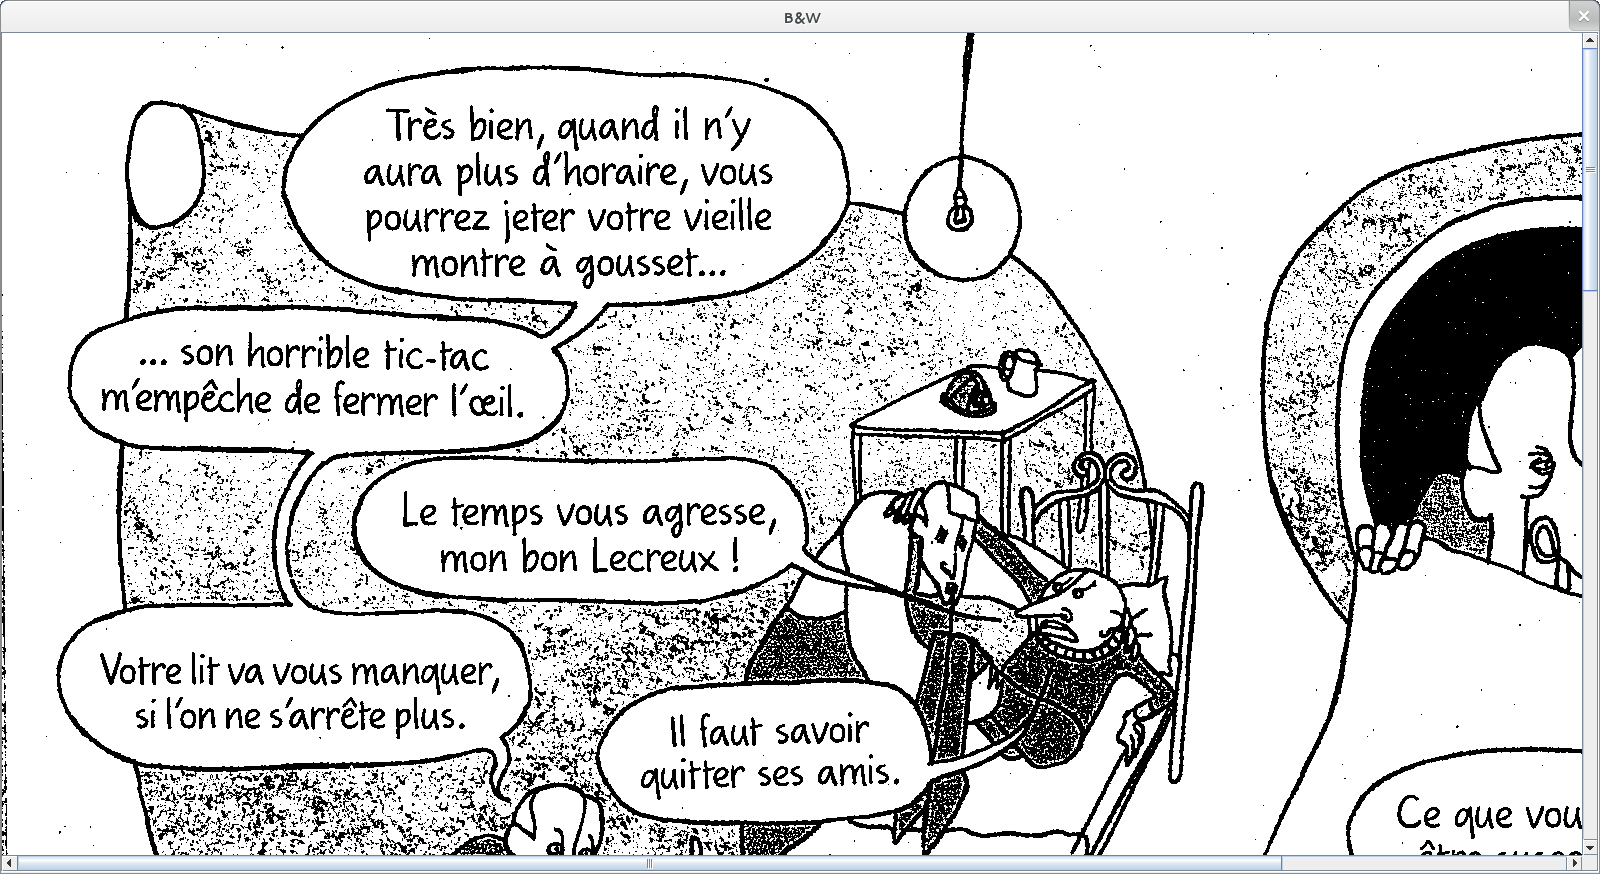
\includegraphics[trim= 597px 20px 500px 400px, clip, width=0.22\textwidth]{bin_200.png}}
	%     \end{array}$
	%   \end{center}
	% \caption[Threshold selection effect]{Segmentation at different threshold levels from the lower top-left to the higher bottom-right (threshold = 50, 100, 150, 200). We observe that the number of CC increases when the dark lines are cut and also when background start to appear as salt and paper noise. Image credits:~\cite{Roudier11}.}
	% \label{fig:in:bin}
	% \end{figure}
	%%%%%%%%%%%%%%%%%%%%%%%%%%%%%%%%%%%%%%%%%%%%%%%%%%%


%Our method, Minimum Connected Components Thresholding (MCCT), automatically finds the right threshold by computing the number of CC for different threshold levels in a range of values from $th_{min}$ to $th_{max}$ and selecting the one that produces the minimum number of CC between the  (in a 8 bits grey image). %We defined a range from 100 to 230 (grayscale value of 8 bits image) for the binarization threshold.
% Our method, Minimum Connected Components Thresholding (MCCT), improves Otsu's threshold selection method by shifting the threshold according to the number of CC that are created.
% Given an Otsu's threshold $th_i$, we segment the image at different threshold centred on $th_i$ (e.g. $th_{i-1}$ to $th_{i-n}$ and $th_{i+1}$ to $th_{i+n}$) and select the one that produces the minimum number of CC (Figure~\ref{fig:in:CC_graph}).
% Note that the threshold selection method requires a single channel image (e.g intensity, luminance) %We defined a range from 100 to 230 (grayscale value of 8 bits image) for the binarization threshold.
% \modif{TODO: experiment and remove $th_{min}$ and $th_{max}$ if possible.}

% Then we find the first minimal number of CC. See example on figure~\ref{fig:in:CC_graph}.
% Note, that the optimal threshold is correctly predicted by MCCT as it corresponds to the bottom-left image figure~\ref{fig:in:bin}.

% 
% 	%%%%%%%%%%%%%%%%%%%%%%%%%%%%%%%%%%%%%%%%%%%%%%%%%%%
	% \begin{figure}[h!]	%trim=l b r t  width=0.5\textwidth,
	%   \centering
	% 	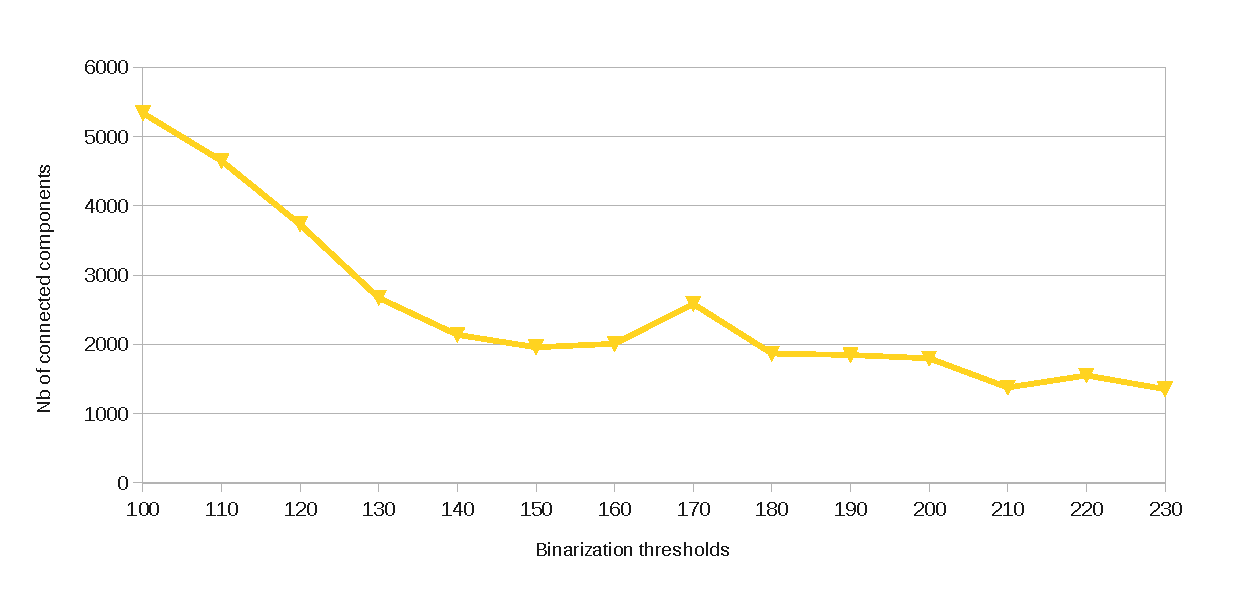
\includegraphics[trim= 0px 0px 0px 0px, clip, width=0.75\textwidth]{CC_graph_source_one_curve.pdf}
	% 	\caption[Evolution of the number of connected-component]{Example of number of CC function of the segmentation threshold. In this case, $th_{min}=100$, $th_{max}=230$ and our algorithm found 150 as optimal threshold threshold \modif{TODO: update with more credible figure from 0 to 255 (average CC evolution instead of single image???)}.}
	% 	\label{fig:in:CC_graph}
	% \end{figure}
% 	%%%%%%%%%%%%%%%%%%%%%%%%%%%%%%%%%%%%%%%%%%%%%%%%%%%

As an alternative segmentation method, we also tried to extract text region using the Maximally Stable Extremal Region (MSER) algorithm~\cite{matas2004robust}.
This algorithm was better than the proposed method only for text region of type onomatopoeia but produced an excess of false detections as in general a lot of the graphical elements are equally stable as the text (flat regions).

% We also try the well known Otsu~\cite{otsu79} algorithm \modif{TODO; justify or delete}.
%\footnote{http://www.labbookpages.co.uk/software/imgProc/otsuThreshold.html}
% (see section~\ref{sec:experiments}).

%Our method is similar to Maximally Stable Extremal Region (MSER) algorithm~\cite{Matas02} because we also try to find an extrema. However, MSER accuracy is low because of the stroke of the text which is very thin compare to the other elements present in the page. This algorithm require a minimum number of stable regions as threshold which as to be very low in our case (text is small region) and a lot of other regions will remain then.

\subsection{Text/graphics separation}
\label{sec:in:textgraphicseparation}
%For the extraction we use CC algorithm for the reason presented in~\ref{sec:segmentation}. We considered only the CC that are black on a white background in the binary image (see figure~\ref{fig:in:bw_wb}). %For the white CC on black background see experiments (section~\ref{sec:experiments}).

After the binary segmentation step we apply the connected-component (CC) labelling method (Section~\ref{sec:ap:connected_component_labelling}) to extract the black strokes as many previous work in the literature (Section~\ref{sec:sota:text}).
At this stage, the extracted components may correspond to part of drawing, single letters or a sequence of letters if some are connected (Figure~\ref{fig:in:detach_attach_letter}).
The objective of this section is to separate the last two categories from the first one.
Note that connected letters will not affect our results (if they are part of the same word) because the expected output is at text line level.


	%%%%%%%%%%%%%%%%%%%%%%%%%%%%%%%%%%%%%%%%%%%%%%%%%%%
	\begin{figure}[h!]%trim=l b r t
	  \begin{center}$
	    \begin{array}{cc}
	     
\includegraphics[height=7mm]{deattached_letter.png} &
	      
\includegraphics[height=7mm]{attached_letter.png}
	    \end{array}$
	  \end{center}
	\caption[Inter-connected letters]{Example of connection between connected components. On the left, a word with six well separated letters, on the right a word detected as two pairs of attached letters because of the handwriting variability and segmentation process.}
	\label{fig:in:detach_attach_letter}
	\end{figure}
	%%%%%%%%%%%%%%%%%%%%%%%%%%%%%%%%%%%%%%%%%%%%%%%%%%%


%The main drawback is when letters are in contact with different lines or drawing elements (see figure~\ref{fig:contact_letter}). We did not work on this assuming that it not so common in comics.

	%%%%%%%%%%%%%%%%%%%%%%%%%%%%%%%%%%%%%%%%%%%%%%%%%%%
% 	\begin{figure}
% 	  \begin{center}$
% 	    \begin{array}{cc}
% 	      \includegraphics[height=15mm]{fig/BW_CC.png} &
% 	      \includegraphics[height=15mm]{fig/WB_CC.png}
% 	    \end{array}$
% 	  \end{center}
% 	\caption{CC black on white (left) and white on black (right) from the same page.}
% \label{fig:in:bw_wb}
% 	\end{figure}
	%%%%%%%%%%%%%%%%%%%%%%%%%%%%%%%%%%%%%%%%%%%%%%%%%%%

%\subsubsection{Letter filtering}

We propose a number of rules, applied sequentially, to separate graphics from text. Due to the wide variety of text usage in comic albums, the method should be size, translation, rotation, scale and contrast invariant. In addition, it should be robust to text-less pages which may appear randomly within an album. From all the components extracted by the CC algorithm, we use three filtering rules to select only the ones corresponding to potential textual elements.

%The idea is to keep only the groups of very contrasted CC.

	%%%%%%%%%%%%%%%%%%%%%%%%%%%%%%%%%%%%%%%%%%%%%%%%%%%
% 	\begin{figure}[!ht]	%trim=l b r t  width=0.5\textwidth,
% 	  \centering
% 		\includegraphics[height=27mm]{fig/contact_letter.png}
% 		\caption{Example of letter in contact with other elements. In this case the bounding box are in blue  (rectangle), in this case of the component 'J' is the whole balloon.}
% 		\label{fig:contact_letter}
% 	\end{figure}
	%%%%%%%%%%%%%%%%%%%%%%%%%%%%%%%%%%%%%%%%%%%%%%%%%%%

% \begin{itemize}

Rule 1: we compare the standard deviation of the grey-levels of the luminance layer of each CC bounding boxes (Figure~\ref{fig:in:std_dev}) with the contrast ratio of the page to make a high/low local contrast CC separation, similarly to~\cite{Li2013Unsupervised} using the Mahalanobis distance~\cite{mahalanobis1936generalized,de2000mahalanobis}.
We assume a Gaussian distribution of the grey level pixels but other distribution are under study. The contrast ratio of the page is the absolute difference between the minimum and the maximum grey-levels found on the page.
% In order to avoid artefacts pixel values, we apply a median filtering as preprocessing.
%The higher the standard deviation is, the higher the probably of being a letter.

%The minimum of difference between letter standard deviation ($\sigma$) and the page content ratio was 1/2 (according to $\sigma=68.27\%$ of the values)

	%%%%%%%%%%%%%%%%%%%%%%%%%%%%%%%%%%%%%%%%%%%%%%%%%%%
	\begin{figure}[h!]
	  \begin{center}$
	    \begin{array}{cc}
	      
\includegraphics[height=10mm]{letter_N_gs.png} &
	      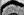
\includegraphics[height=10mm]{letter_eyeblow_gs.png}
	    \end{array}$
	  \end{center}
	  \caption[Mean and standard variation values of connected-component bounding boxes]{Example of mean ($\mu$) and standard deviation ($\sigma$) values of two CC bounding box regions. For the letter ``N'',  $\mu,\sigma=[167,84]$ and for the eyebrow $\mu,\sigma=[110,57]$. %In this case the contrast ratio of the page was 255, N is high contrasted 2$\sigma > 255 * 50\% $ unlike the eyebrow.
	  }
	  \label{fig:in:std_dev}
	\end{figure}
	%%%%%%%%%%%%%%%%%%%%%%%%%%%%%%%%%%%%%%%%%%%%%%%%%%%

% Rule 2: we apply a topological filtering that consists in removing all the CC that overlap with others assuming that the CC of a letter can not contain another CC, similar to~\cite{Kasar07}.
% In our study we consider only the black on white CC (Figure~\ref{fig:in:bw_wb}).

% 	%%%%%%%%%%%%%%%%%%%%%%%%%%%%%%%%%%%%%%%%%%%%%%%%%%%
% 	\begin{figure}[h!]%trim=l b r t
% 	  \begin{center}$
% 	    \begin{array}{cc}
% 	      
\includegraphics[height=8mm, trim= 0px 4px 0px 3px, clip]{BW_bin_CC.png} &
% 	      
\includegraphics[height=8mm, trim= 0px 4px 0px 3px, clip]{WB_bin_CC.png}
% 	    \end{array}$
% 	  \end{center}
% 	\caption[Difference between black over white and white over black connected-components]{On the left, an example of black over white CC bounding box (red rectangle) and on the right side, a white over black (the white inside region of the letter ``A'').}
% 	\label{fig:in:bw_wb}
% 	\end{figure}
% 	%%%%%%%%%%%%%%%%%%%%%%%%%%%%%%%%%%%%%%%%%%%%%%%%%%%


Rule 2: we verify that each letter $l_i$ is surrounded by other letters $l_j$ (with $_j\in{[0,n]}$) which is intrinsic to the design of text (grouping characters in words and text lines).
To do so, we check for similar in height components in a local region equal to the size of the component's bounding box extended to its left/right/top/bottom directions (Figure~\ref{fig:in:4_direction}). For instance, $l_i$ is considered similar in height to $l_i$ if $abs(l_i.height - l_j.height)<a*l_i.height$ ($a=$similarity offset). %If yes then both are considered as letter.
%\end{enumerate}


	%%%%%%%%%%%%%%%%%%%%%%%%%%%%%%%%%%%%%%%%%%%%%%%%%%%
	\begin{figure}[h!]	%trim=l b r t  width=0.5\textwidth,
	  \centering
		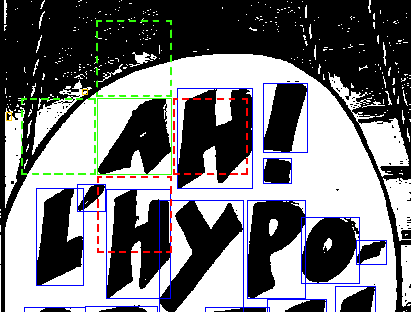
\includegraphics[width=0.50\textwidth]{4_direction.png}
		\caption[Text candidate region neighbourhood analysis]{Neighbourhood analysis for text and non text classification (rule 3). The area of the bounding box of the letter ``A'' is extended in four directions around the letter ``A'' to check if any other letter (blue rectangles) overlaps with it. In this example, there are two overlapping components (red dashed rectangles) at the right and the bottom of the letter ``A''. The component is thus accepted as a text letter candidate.}
		\label{fig:in:4_direction}
	\end{figure}
	%%%%%%%%%%%%%%%%%%%%%%%%%%%%%%%%%%%%%%%%%%%%%%%%%%%

Rule 3:
we check all the CC bounding boxes pairs that overlap more than $b$\% each other.
We remove the biggest from each pairs.

\subsection{Text line generation} % (fold)
\label{sub:in:text_line_generation}
As already mentioned Section~\ref{par:se:letter_to_line}, the gap between text component (e.g. letter or attached letters, word) and text lines can vary significantly.
Here we use the same method as presented in Section~\ref{par:se:letter_to_line} to group text component into text lines considering only the text height (or width for vertical text).
%We can group text parts to text lines using the method presented Section~\ref{par:se:letter_to_line}.

% subsection text_line_generation (end)
% \end{itemize}


\subsection{Text recognition} % (fold)
\label{sub:in:text_recognition}
Automatic text recognition has been studied for many years, today OCR systems are very efficient for standard fonts but not optimized for comics fonts which are mostly handwritten.
The principal interest of text recognition is the ability of searching images by using keywords which opens up many applications (Section~\ref{sec:sota:text}).
Text recognition applied to comics is really challenging because it includes most of the difficulties from text recognition in document analysis domain if we consider all the type of text that composed the comics.
From typewritten to handwritten and free-form text in uniform to complex background including image noise, text deformation and overlapping (Figure~\ref{fig:in:texlines_example}).
Note that the text is mainly written in upper case for Latin scripts in comics which reduce the complexity of recognition.

%%%%%%%%%%%%%%%%%%%%%%%%%%%%%%%%%%%%%%%%%%%%%%%%%%%
 \begin{figure}[!ht]  %trim=l b r t  width=0.5\textwidth,
   \centering
  \fbox{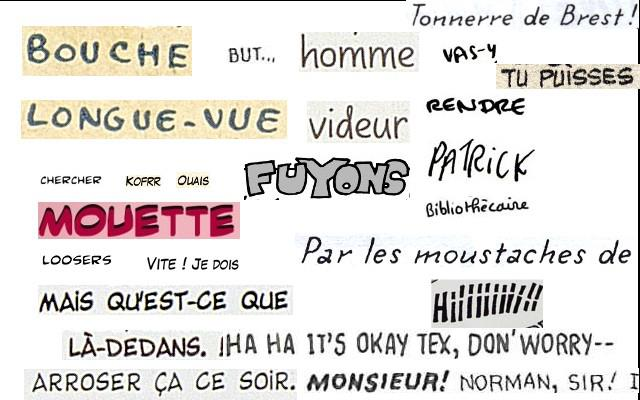
\includegraphics[trim= 1px 1px 3px 2px, clip, width=0.75\textwidth]{text_line_examples.png}}
  \caption[Examples of text lines from comics images]{Examples of text lines from comics images.}
  \label{fig:in:texlines_example}
 \end{figure}
%%%%%%%%%%%%%%%%%%%%%%%%%%%%%%%%%%%%%%%%%%%%%%%%%%%

% Text recognition in comics would allow full-text search, tagging, image description, comic character labelling etc.
Text recognition for comics requires an extensive work to be addressed properly, which is out of the scope of this thesis work.
Even if standard OCR recognition rate is not yet acceptable yet for full-text based application in comics, they can help at separating text/non text regions.

We pass each text line candidate through an OCR system to validate its content.
The validation criterion is that the OCR recognize at least one alphabetical symbol within the candidate region, else it is rejected.
The text line are composed by 12 character in average which give a good chances to OCR to recognize at least one of them (Section~\ref{sec:dataset_description}).


% Nevertheless, we measure the performance of current OCR systems Section~\ref{sub:ex:text_extraction_recognition_evaluation}.

% section text_localisation_and_recognition (end)

\section{Balloon extraction and classification}
\label{sec:in:balloon}

In this section we present a method for pixel level balloon extraction and for balloon classification.
Balloon extraction does not requires previous text extraction unlike the method presented Section~\ref{sub:se:regular_balloon_extraction} but uses a careful analysis of the region content (e.g. similarities, spacial organisation) to predict which are most likely balloon regions.
Balloon contour and shape information differences are presented and a contour-based classification method is detailed for ``smooth'', ``wavy'' and ``zigzag'' classes that may correspond to ``dialogue'', ``thought'' and ``exclamation'' in a higher level context (\ch{chap:knowledge}).

\subsection{Balloon segmentation} % (fold)
\label{sub:in:balloon_segmentation}
From the reviewed methods Section~\ref{sec:sota:balloon_segmentation}, we can see that the text position often help in the localization and then segmentation of speech balloons.
The issue in relying on text extraction is that we become dependent of its performance.
The text extraction in comics images is still a challenging problem (Section~\ref{sec:in:text_localisation_and_recognition}), it is a very hard assumption to assume the text extraction will work perfectly. 
% two of them~\cite{Ho2012,rigaud2013active} are based on text position which relies on the text extractor performance.
Instead of relaying on the text detection we propose to keep both processes independent in order to avoid errors of propagation.
% independent the low level processing.
In a similar way, Arai's method~\cite{Arai11} does not use text position but connected component filtering based on heuristics (fixed thresholds for binary image segmentation, blob size, number of white pixels, number of contained straight lines and width to length ratio). 
We propose a more adaptive method in order to handle various comics styles (e.g. colour, B\&W), image formats (e.g. A4, A5, portrait, landscape) and digitization variations (e.g. scanning device, camera capture).

The use of fixed thresholds for the segmentation process such as~\cite{Arai11} is a strong assumption about the image background nature.
It only works for comics from the same style and digitized under the same light condition.
We propose to relax the constraint by using Otsu's threshold selection method~\cite{otsu79} to make a global binary segmentation of the grey-scale image.
The binary segmentation creates a lot of small connected components on textured images, we prune it by removing the connected components that are classified as ``noise'' by the algorithm presented Section~\ref{sec:se:panel_and_text}.
%~\cite{Rigaud2012LNCS} (class with the minimum average height).
% and then we add one time the standard deviation value to avoid opening black contour by choosing a low threshold such as~\cite{.
We extract connected components from the binary image and analyse their parent-child relationship to make a first selection of candidate components and then analyse the spatial organisation of the set of children $CH=\{ch_1, ch_2,...,ch_n\}$ to compute a confidence value for each parent $P=\{p_1, p_2,...,p_m\}$ that serve as final filtering criterion (Figure~\ref{fig:in:balloon_binarisation}).

%%%%%%%%%%%%%%%%%%%%%%%%%%%%%%%%%%%%%%%%%%%%%%%%%%%
 \begin{figure}[!ht]  %trim=l b r t  width=0.5\textwidth,
   \centering
  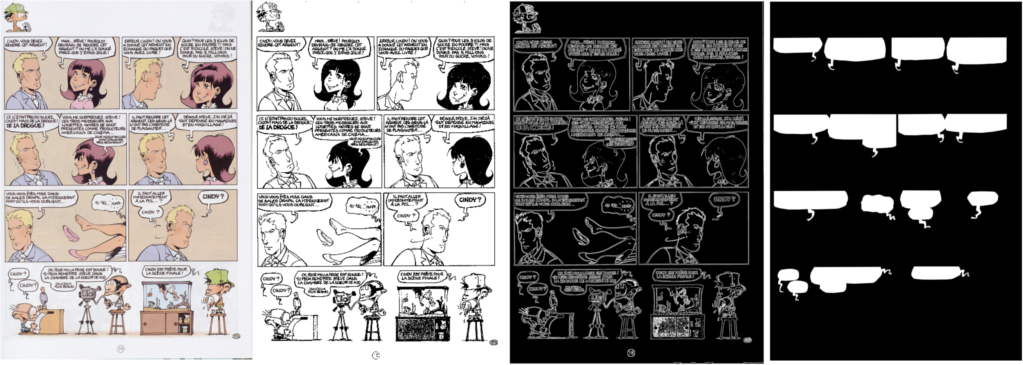
\includegraphics[width=0.9\textwidth]{closed_balloon_process.png}
  \caption[Balloon extraction process]{Balloon extraction process. Original image, binary segmentation, contour detection (connected components) and result mask from left to right.}
  \label{fig:in:balloon_binarisation}
 \end{figure}
%%%%%%%%%%%%%%%%%%%%%%%%%%%%%%%%%%%%%%%%%%%%%%%%%%%

We assume that a balloon has a minimum of children $minNbChildren$ which are horizontally or vertically aligned and centred inside the balloon region (property of text).
The percentage of alignment $align$ is computed for each child $ch_i$ considering $CHA(ch_i)$ the subset of children that are aligned to $ch_i$ (Equation~\ref{eq:in:balloon_alignment}).

\begin{equation}
	\label{eq:in:balloon_alignment}
	align(ch_i) = \frac{|CHA(ch_i)|}{n}
\end{equation}
where $|CHA(ch_i)|$ is the number of aligned children and $n$ the total number of children.

%TODO: Dimos on 2014-06-30: use a min criteria isAligned IF more than N=4 chidlen are aligned with the current one + decide the percentage of children that are valid over all the children of the parent -> confidence value.

For instance, if we consider two children $E$ and $F$, they are considered as aligned (vertically) if the following conditions are verified $centroidF_x \in [minE_x, maxE_x]$ and $centroidE_x \in [minF_x, maxF_x]$ where $min_x$ and $max_x$ are the left and right limits on the horizontal axis.
The child $F$ is also considered to be aligned (horizontally) to $E$ by changing $x$ to $y$ which become the top and bottom bounding box limits.

We use the difference of alignment between the balloon candidate and its children as a clue about its probability of being a real balloon in image.
This is similar to the text dependent balloon extraction method presented Section~\ref{sec:se:panel_and_text}.
The difference is that here we have no idea about the nature of the children (not detected as text before).
This independent balloon extraction method can be seen as an ``intelligent'' balloon extractor that embeds a part of a the domain knowledge related to text (balloons are expected to contain text).
The difference of alignment is computed for the horizontal ($d_x$) and the vertical ($d_y$) axis from the Euclidean distance between the parent and children hull centroids (Figure~\ref{fig:in:coaxial_alignment}).


    %%%%%%%%%%%%%%%%%%%%%%%%%%%%%%%%%%%%%%%%%%%%%%%%%%%%%%%%
    \begin{figure}[ht]%trim=l b r t  width=0.5\textwidth,  
      \centering
      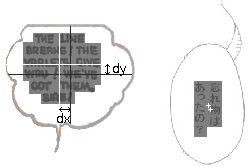
\includegraphics[trim= 0px 15px 80px 24px, clip, width=0.35\textwidth]{coaxial_alignment.png}
    \caption[Balloon content alignment measures]{Horizontal and vertical alignment measurement between the centroids of the balloon (dark cross) and the children hull (clear cross). The children hull is the grey region included in the balloon.}
    \label{fig:in:coaxial_alignment}
    \end{figure}
    %%%%%%%%%%%%%%%%%%%%%%%%%%%%%%%%%%%%%%%%%%%%%%%%%%%%%%%%

Both differences $d_x$ and $d_y$ are normalized between zero and one as a percentage of the balloon (parent) width and height respectively.
The average of the alignments, $\overline{align}$, $d_x$ and $d_y$ gives a confidence value for each candidate of $P$ (Formula~\ref{eq:in:balloon_confidence_value}).

\begin{equation}
	\label{eq:in:balloon_confidence_value}
	C_{balloon} = \frac{1}{3} * \Big( \overline{align} + d_x + d_y \Big)
\end{equation}

The confidence value is used for balloon and non balloon decision (Section~\ref{sub:ex:balloon_extraction_evaluation}).
%TODO: justify the product with fuzzy logic approaches for information combination

% This work have been submitted to the International Journal on Document Analysis and Recognition~\ref{???}.

Tail detection is not treated as an independent extraction because it is part of balloons and never appears without being related to a regular or implicit balloon.
Please refer to Section~\ref{sec:se:from_balloon_to_tail} for more detail about tail detection.

\subsection{Balloon classification} % (fold)
\label{sub:in:balloon_classification}

Speech balloon classification is a real challenge if we consider a lot of different comics styles.
First, each author has his own representation of the speech sounds. Second, the reader interpretation is subjective (each balloon style is interpreted in comparison to the already read balloon styles).
For those reasons, it is really hard to directly define the purpose (e.g. dialogue, thought and exclamation) of a speech balloon without knowing its context in the story.
In fact, the context is defined by both graphic (e.g. other strokes, protagonists personality) and textual (e.g. vocabulary, punctuation) elements.
For instance, Figure~\ref{fig:in:contour_style} shows six different speech balloon comics styles where we can note the difficulty to assign one class for each balloon without knowing others balloon shapes and reading the contained text.

% Note, speech balloon classification is complementary to speech balloon extraction that has already been studied using white connected component extraction and filtering~\cite{Arai11,Ho2012} or active contour model~\cite{Rigaud2013ICDAR}.


	%%%%%%%%%%%%%%%%%%%%%%%%%%%%%%%%%%%%%%%%%%%%%%%%%%
	\begin{figure}[!ht]	%trim=l b r t  width=0.5\textwidth,
	  \centering
		\fbox{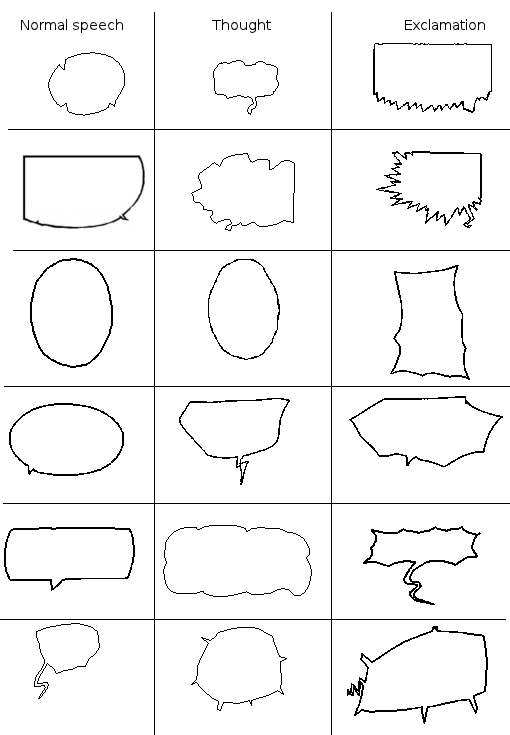
\includegraphics[trim = 0mm 1mm 0mm 0mm, clip, width=0.8\textwidth]{contour_style.png}}
		\caption[Relation between speech balloon shape and contour informations]{Examples of speech balloons from 6 comics albums (rows) that represent 3 different expressions (columns).}
		\label{fig:in:contour_style}
	\end{figure}
	%%%%%%%%%%%%%%%%%%%%%%%%%%%%%%%%%%%%%%%%%%%%%%%%%%


% Balloon classification aims to automatically determine which balloons are for normal speech, though and exclamation.
% This information add a new level of understanding of the comics image content.
% From our knowledge, speech balloon classification has not been studied before.
% It is related to contour classification in planar images.



% \subsubsection{Proposed method}
% \label{sec:in:contour_classification}

The input of the proposed method is a pixel-level balloon contour detection, such as proposed in Sections~\ref{sub:se:regular_balloon_extraction} and~\ref{sec:in:balloon}.

The shape and the contour of a balloon contain different type of information.
The shape (e.g. rectangle, square, circle, oval) does not provide a lot of information about how the text is spoken, it is more related to the style of the comics and the structure of the panel.
However, the contour contains the speech tone information according to the different patterns which are along the boundary of the balloon.

% In this section we detail how we perform the shape and contour separation, the contour description and finally the classification using a Bayesian classifier.

% The next section details the balloon shape/contour information separation, description and classification.
% Section~\ref{sec:experiments} evaluates the proposed method by showing the results of speech balloon classification.
% Finally, section~\ref{sec:discussion} and~\ref{sec:conclusion} discuss and conclude this work.


\subsubsection{Shape/contour separation}
\label{sec:contour_detection}
As introduced in Section~\ref{sec:sota:balloon_segmentation}, the discriminant information for speech balloon classification is not provided by the global shape but by the contour variations. 

First, we propose to represent the speech balloon as a time series (one dimensional signal over $360^\circ$) which corresponds to the distance in number of pixels between the balloon barycentre and the contour points. 

Second, we perform a shape/contour separation to be able to analyse only the contour variation (including the balloon tail). We approximate the global shape $s$ by smoothing the original signal $o$ using a sliding window of size $M$ and subtracting the result from the original signal to preserve only the contour information $c$ independently from the shape: $c = o - s$. The smoothed contour $s$ is a centred local average of $o$ (Formula~\ref{eq:be:smooth}).
Examples are given Figure~\ref{fig:be:time_series}.

% and normalized by the letter height $\bar{H}$ (see eq.~\ref{eq:avg_height}).

	%%%%%%%%%%%%%%%%%%%%%%%%%%%%%%%%%%%%%%%%%%%%%%%%%%
	\begin{figure}[!ht]	%trim=l b r t  width=0.5\textwidth,
	  \centering
		\fbox{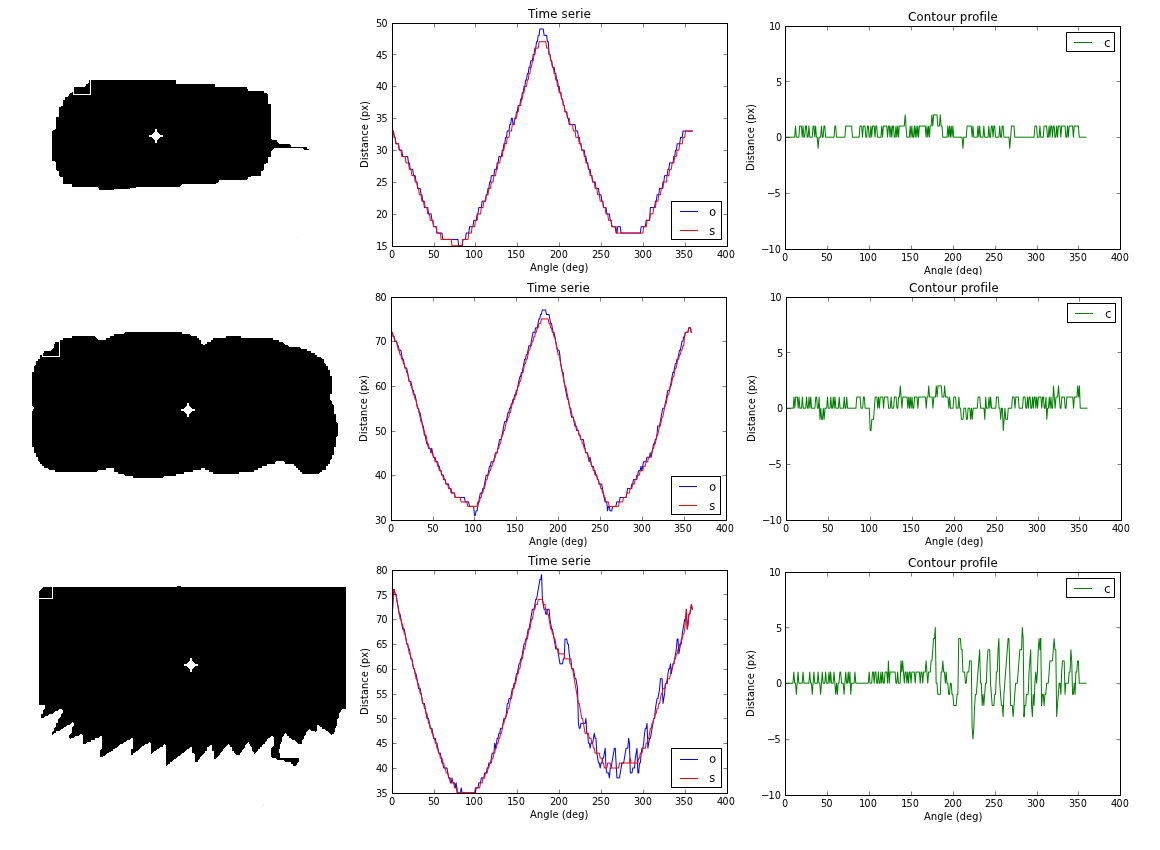
\includegraphics[ width=0.9\textwidth]{time_series.png}}
		\caption[Balloon contour time series]{Balloon detection, time series representation and shape/contour separation. Left column represents balloon detection with the barycentre (white hole) and the starting point (top left half square). Middle column represents the distance between the barycentre and the balloon boundary over $360^\circ$ (clockwise) where the original signal $o$ is in blue and the smoothed signal $s$ in red. Right column is the difference between $s$ and $o$.}
		\label{fig:be:time_series}
	\end{figure}
	%%%%%%%%%%%%%%%%%%%%%%%%%%%%%%%%%%%%%%%%%%%%%%%%%%

\begin{equation}
\label{eq:be:smooth}
 s(o) = \frac{1}{M} * \sum_{-M/2}^{+M/2} o
\end{equation}
% where $M$ is the window size.% For instance, if $M=10$ and $i=20 \in[0, 360]$, $s_{20}$ will be the average of the distances between $o_{15}$ to $o_{25}$.



\subsubsection{Contour description}
\label{sec:be:description}
%In this section we propose a method to classify speech balloon contours by using time series representation. %An alternative could be based on the center of mass~\cite{Keogh2006}.

Contour description encodes the contour variations relatively to the balloons size to be invariant to page format and definition.

The level of variation can be computed from different features, the main difficulty is to be invariant to the comics drawing diversity. 
In this study, we describe the contour signal $c$ by using a variance-based two dimensional descriptor, more precisely the standard deviation $\sigma$. The variance or the standard deviation have the advantage to be simple and generic at describing any data distribution by measuring the data dispersion which is what we need if we aim at measuring the difference of dispersion between the original and the smoothed contours. In order to be invariant to the image definition and scale, we normalize each feature of the descriptor by the original signal average $\bar{o}$ (average radius).
%The first dimension is the global contour signal variance and the second is the difference between the top and bottom part variances. 

The first dimension aims to differentiates contours which have high variations (``zigzag'' type) from the others (``wavy'' and ``smooth'' types). The second dimension aims to discriminate ``wavy'' and ``smooth'' types according to the standard deviation of the superior and inferior signal part from the average $\bar{c}$. For instance, if a contour has a higher standard deviation in the below signal part than the above signal part (according to the average $\bar{c}$) then the contour has more peaks in the direction of its barycentre than the opposite, which is not a characteristic of the ``smooth'' type but ``wavy''.

The first feature $f_1$ consists in measuring the standard deviation $\sigma_c$ of the contour signal $c$ normalized by the original signal average $\bar{o}$ (Formula~\ref{eq:be:distortion}).


\begin{equation}\label{eq:be:distortion}
 f_1 = \frac{\sigma_c}{\bar{o}}% * \sum_{i=-M/2}^{+M/2} o
\end{equation}
where $f_1$ is the feature one, $\sigma_c$ the contour standard deviation normalized by $\bar{o}$ the average of the signal $o$. 


In order to measure the second feature $f_2$, we split the contour signal $c$ in two signals $c_{pos}$ and $c_{neg}$ which correspond to the signal parts that are strictly above and below the average $\bar{c}$ (Figure~\ref{fig:be:signal_decomposition}) and then we measure the standard deviation differences (Formula~\ref{eq:be:var_diff}).% compares the superior and inferior variances of the contour signal average $\bar{c}$


\begin{equation}\label{eq:be:var_diff}
 f_2 = \frac{\sigma_{neg} - \sigma_{pos}}{\bar{o} }% * \sum_{i=-M/2}^{+M/2} o
\end{equation}
where $f_2$ is the feature two, $\sigma_{pos}$ and $\sigma_{neg}$ are the standard deviations of the signals $c_{pos}$ and $c_{neg}$ respectively. The difference is normalized by $\bar{o}$.% a contour descriptor, $v$ the contour variance and $\bar{o}$ the average of the signal $o$. 


	%%%%%%%%%%%%%%%%%%%%%%%%%%%%%%%%%%%%%%%%%%%%%%%%%%
	\begin{figure}[!ht]	%trim=l b r t  width=0.5\textwidth,
	  \centering
		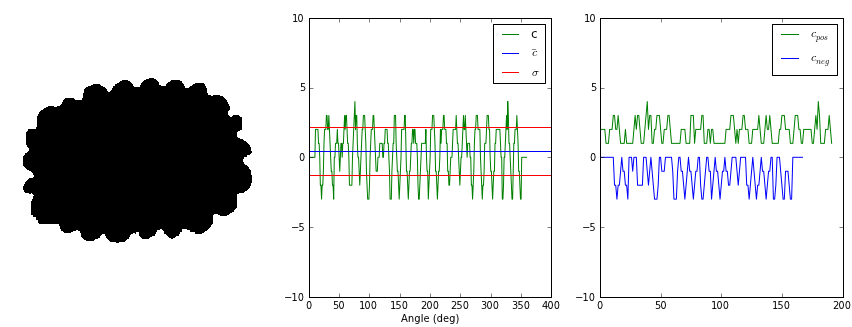
\includegraphics[trim = 0mm 0mm 0mm 0mm, clip, width=340px]{signal_decomposition.png}
		\caption[Contour signal decomposition]{Contour signal decomposition. Left part is the concerned speech balloon, middle part is its contour profile and right part is the positive and negative decomposition according to the contour average $\bar{c}$. Both signal have not the same length because we ignore values that are equal to the average value $\bar{c}$ in order to not bias the standard deviation.}
		\label{fig:be:signal_decomposition}
	\end{figure}
	%%%%%%%%%%%%%%%%%%%%%%%%%%%%%%%%%%%%%%%%%%%%%%%%%%


\subsubsection{Contour classification}
Contour classification is performed according to the selected contour descriptor (Section~\ref{sec:be:description}) by using a naive Bayesian Classifier~\cite{Mitchell1997}.
This classifier has been chosen because it requires a small amount of training data.
Let a label set $L=(l_1,l_2,l_3)$ represent the three contour classes ``smooth'', ``wavy'' and ``zigzag''. Given a new unlabelled contour $c$ described by its descriptor $D=(f_1,f_2)$, the naive Bayes approach assigns $D$ to a class $l_{MAP}$ as follow:

\begin{equation}\label{eq:be:fine_class}
  l_{MAP} \\
  = \mbox{argmax}_{l} P(l|D) \\
  = \mbox{argmax}_{l} \frac{P(l) P(D | l)}{P(D)}\\
  = \mbox{argmax}_{l} P(l) P(D | l)
\end{equation}
where $P(l)$ is the \textit{a priori} probability of class $l$ and $P(D|l)$ is the conditional probability of a given descriptor $D$ to be in the class $l$. This conditional probability follows a Gaussian distribution for which we learn the parameters during the training step.


% This work have been submitted to the Tenth IAPR International Workshop on Graphics Recognition~\cite{RigaudGREC2013} and extended in the a chapter of the Graphics Recognition book~\ref{???} (Lecture Note in Computer Science).

% subsection classification (end)



\section{Comic character spotting}
\label{sec:in:character_spotting}
% This section introduces a supervised character spotting method based on that requires only one rough example of the protagonist for which we are interested in to retrieves all the other instances.
% This colour-based approach... 
Human detection in computer vision field is an active field of research. Extending this to human-like drawings such as the main characters in comic book stories is not trivial.
% Comics analysis is a very recent field of research at the intersection of graphics, texts, objects and people recognition.
The detection of the main comic characters is an essential step towards a fully automatic comic book understanding.
This section presents a colour-based approach for comics character spotting using content-based drawing retrieval and colour palette descriptor.

In this section we detail how to localize comics characters in all pages of a given album.
We aim at detecting the apparitions of a comics character (non-rigid object) with a minimum of user interaction. This is a content based image retrieval problem where the result highly depends on the quality of the given example, that should be noise free (no background, target only). 
A close up view of comics drawings shows that the most invariant information between texture, shape and colour is the colour information. We believe that this feature is the only information which is invariant to scale, object deformation, translation and rotation transformations which are very frequent in comics. The typical drawback of using colour features is that they are sensitive to illumination and contrast variations. This is an important issue for natural images but not for hand drawings if they are drawn and digitized under the same conditions. 

For all those reasons we based our method on colour information only.
Given a comic page, we first ask the user about the position of one object example and then we perform and exhaustive search in all the pages of the same album or collection.
% crop the query character at pixel level or select manually only desired pixels but we propose to speed up the process by cropping two different characters (rectangle bounding box) containing two different apparitions of the object. 
%We preferred to ask the user a minimum of interaction by manually localizing two objects and then compute automatically the colour descriptor instead of manually describe the colour image. 
%The idea is to compare both image crops and automatically remove colours that do not belong to the object (background colours).
%Note, the colour selection has to be carefully done to avoid background details.

The proposed method can be summarized as follows (for a given comics album) :
\begin{itemize}
  \item Compute and apply a reduced colour palette to all pages
  \item Get the object colours from input query
  %\item select query colours (most representative colours)
  \item Compute the query descriptor
  \item Retrieve similar objects
\end{itemize}

The retrieval (search) step can be extended to other albums from the same collection (similar comics characters).
 


%------------------------------------------------------------------------
\subsection{Colour quantization}
Once the user has highlighted the query region, we reduce the number of colour of all the images of the album (including the query region) according to a colour palette $P_c$.
Colour reduction or quantization generally involves two steps.
The first step is to choose a proper colour palette and the second step is to reconstruct an image by replacing original colours with the most similar colour from the palette.

% \modif{TODO: Il faut donner les détails de la méthode que tu utilises sauf si tu l'as mise dans l'état de l'art au chapitre 2 (faire lien).
%Describe method and propose L0-smoothing ++ as promising alternative but the chosen method is simple, faster and good enough for our purpose. RGB colour space?}

Before quantizing the image colours, we smooth the image in order to reduce the impact of printed dithering effects that sometimes appear during the printing and scanning process and obtain flat colours.
We use a state of the art method of Kopf that shown very good results on comics images~\cite{Kopf2012DigitalReconstruction} (Figure~\ref{fig:in:smoothing_quantization}).

The colour palette $P_c$ is computed from the $N$ most frequent colours in the album and then each pixel is changed by its most similar colour from the palette to produce the quantized image.

This limited amount of colours allows to describe and retrieve the object with only few representative colours.


  %%%%%%%%%%%%%%%%%%%%%%%%%%%%%%%%%%%%%%%%%%%%%%%%%%%
  \begin{figure}[h!]  %trim=l b r t  width=0.5\textwidth,
    \centering
    
\includegraphics[trim= 0px 0px 0px 0px, clip, width=0.75\textwidth]{figure_here.png}
    \caption[Colour image smoothing and quantization for comic character extraction]{Colour image smoothing and quantization effects for comic character extraction (3 columns, original, l0-smoothed, corresponding 256 palette).}
    \label{fig:in:smoothing_quantization}
  \end{figure}
  %%%%%%%%%%%%%%%%%%%%%%%%%%%%%%%%%%%%%%%%%%%%%%%%%%%


% An alternative would be to compute a more specific palette according to the query colours.


%------------------------------------------------------------------------
\subsection{Input query}
\label{sec:in:input_query}
A minimal user interaction is necessary to tell the system what to retrieve in the album or collection.
We only ask the user to give an information about the object's colours by selecting few pixels from the query object.
We propose to use a pointing device (e.g. mouse, finger on touchscreen) to click, drag and release over the object colours and make the selection of pixels (Figure~\ref{fig:in:user_selection}).
This selection can be assisted using a scribble-based tool~\cite{Xu2012LazySelection}.

%%%%%%%%%%%%%%%%%%%%%%%%%%%%%%%%%%%%%%%%%%%%%%%%%%%
 \begin{figure}[!ht]	%trim=l b r t  width=0.5\textwidth,
 	 \centering
 	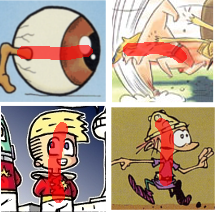
\includegraphics[width=0.5\textwidth]{user_selection.png}
 	\caption[User defined comics character selection]{Examples of comics character colour selection using a pointing device (click, drag and release). Selected pixels are highlighted in red, they constitute the query given by the user.}
 	\label{fig:in:user_selection}
 \end{figure}
%%%%%%%%%%%%%%%%%%%%%%%%%%%%%%%%%%%%%%%%%%%%%%%%%%%

%------------------------------------------------------------------------
\subsection{Query descriptor}

The query descriptor we use is a non ordered colour vector that contains the information of presence of certain colours in the query ($D \subset P_c$). It is not composed by spatial or quantitative information (e.g. region positions, number of pixels) because these parameters are not scale and deformation invariant.% The integration of these spatial information is the object of current research in our research group.

% -------------------------------------

% The ROIs computed by the expert system are less accurate than the one given by the user in~\cite{RigaudDAS2014}, it may cut a part of the character and contains more pixels from background than from the comics character (see figure~\ref{fig:query_user_expert}).
% Computing the query descriptor directly from the region proposed by the expert system would result in considering a lot of information that is not part of the character (noise).
% We need to remove background information first and then describe the query region.
% We propose to automatically find the $N$ more discriminant hue values of the character from the hue values that are inside but not outside the expected region in the panel.
%This can be formalized as a TF-IDF~\cite{salton1986introduction} (Term Frequency - Inverse Document Frequency).
% The application of classical TF-IDF~\cite{salton1986introduction} numerical statistic to hue values allows us to identify the importance weights of the different hue value in the query image.
%We propose then to combine the inverse term frequency and the document frequency in order to highlight the transcriptions that are not frequent in a single page but that constantly appear in invoices from the same provider. 
%Given a word transcription w and a document set d, the itf-df weight is computed as:
% In our application, the {\it term frequency} $(tf)$ corresponds to the ratio of pixels of a particular hue value $h_i$ in the set of hue values that compose the query region $qH=\{h_0, h_1,...,h_n\}$.% over the number of pixel in the query region $q$.
% The {\it inverse DOCUMENT frequency} $(idf)$ corresponds, for a given hue value $h_i$, to the logarithm of the total number of pixel in the panel $|p|$ (corpus) over the number of pixel of hue value $h_i$ in the panel $|p| \cup |h_i|$.
% The score for each hue value $h_i$ in $qH$ corresponds to $tf_i * idf_i$ and the $N$ hue values that correspond to the $N$ highest scores are used to define the colour descriptor $D=\{h_0,h_1,...,h_N\}$.
% See equation~\ref{eq:query_colors_tf},~\ref{eq:in:query_colors_idf} and figure~\ref{fig:color_filtering}.

% %The query descriptor $D$ is a set of $N$ hue values $D=\{h_0,h_1,...,h_N\}$.

% % % tf = float(nbPixelMatchInQnbPixInQueryy
% % % idf = math.log(float(nbPixInPanel) / nbPixelMatchInPanel)

% % %scores val = tf * idf

% \begin{equation}
%    %tf = \frac{nbPixelMatchInQuery}{nbPixInQuery}
%    tf = \frac{nbPixelMatchInQuery}{nbPixInQuery}
%    \label{eq:query_colors_tf}  
%   \end{equation}

% \begin{equation}
%  idf = \log \frac{nbPixInPanel}{nbPixelMatchInPanel}
%    \label{eq:in:query_colors_idf}  
%   \end{equation}

%%%%%%%%%%%%%%%%%%%%%%%%%%%%%%%%%%%%%%%%%%%%%%%%%%%
 % \begin{figure}[!ht]  %trim=l b r t  width=0.5\textwidth,
 %   \centering
 %  \includegraphics[trim= 0px 75px 0px 0px, clip, width=240px]{fig/masks.png}
 %  \caption{Original panel with the query (blue rectangle) and the corresponding hue value histogram in the query region and non query region from top to bottom.% Each image has its corresponding histogram of hue values normalized between 0 and 255 on the right hand side.
 %  %The bar graph in the bottom part represents the hue values that are present in the inside ROI but not in the outside ROI histograms.
 %  }
 %  \label{fig:color_filtering}
 % \end{figure}
%%%%%%%%%%%%%%%%%%%%%%%%%%%%%%%%%%%%%%%%%%%%%%%%%%%

% Once the discriminant colours are extracted, we build the query descriptor $D$ from the $N$ most important colours.

% -----------------------------------------------

\modif{TODO: use Hue instead of colour quantization = experiment more}

The colour subset $D$ is composed by the $N$ colours the most represented in the query region and that are the most discriminating in the image or collection.
We define two metric for each colour of the query region in order to determinate which ones will be used for the query description.
The first metric $L_{1c}$ corresponds to the number of pixel of a colour $c$ in the query region (colour histogram Figure~\ref{fig:in:dominant_colour_hist_desc}) and $L_{2c}$, the discriminability level of the colour $c$ in the whole image.

The discriminability level can be formalized as a TF-IDF~\cite{salton1986introduction} (Term Frequency - Inverse Document Frequency) numerical statistics that allows us to identify the importance weights of the different colour value in the query image.
In our application, the {\it term frequency} $(tf)$ corresponds to the ratio of pixels of a particular hue value $h_i$ in the set of hue values that compose the query region $qH=\{h_0, h_1,...,h_n\}$.% over the number of pixel in the query region $q$.
The {\it inverse document frequency} $(idf)$ corresponds, for a given hue value $h_i$, to the logarithm of the total number of pixel in the image $|p|$ (corpus) over the number of pixel of hue value $h_i$ in the image $|p| \cup |h_i|$.
The score for each hue value $h_i$ in $qH$ corresponds to $L_{2c_i} = tf_i * idf_i$ and the $N$ hue values that has the $N$ highest scores are used as colour descriptor of the query region $D=\{h_0,h_1,...,h_N\}$.
See Equations~\ref{eq:query_colors_tf},~\ref{eq:in:query_colors_idf}.% and figure~\ref{fig:color_filtering}.

%The query descriptor $D$ is a set of $N$ hue values $D=\{h_0,h_1,...,h_N\}$.

% % tf = float(nbPixelMatchInQnbPixInQueryy
% % idf = math.log(float(nbPixInPanel) / nbPixelMatchInPanel)

% %scores val = tf * idf

\begin{equation}
   %tf = \frac{nbPixelMatchInQuery}{nbPixInQuery}
   tf = \frac{nbPixelMatchInQuery}{nbPixInQuery}
   \label{eq:query_colors_tf}  
  \end{equation}

\begin{equation}
 idf = \log \frac{nbPixInImage}{nbPixelMatchInImage}
   \label{eq:in:query_colors_idf}  
  \end{equation}

The discriminability level $L_{2c}$ allows us to ignore colours that are not only dominant in the query region but also in the rest of the image.
For instance, black and white colours are often in the query region but also in many contour and background regions which will not help the retrieval process if we include them in the query description (not discriminant colours).

Each value of $L_{1c}$ and $L_{2c}$ are normalized as a percentage between 0 and 1, the score for each colour is the average of both term: $Score(c) = 1/2 * (L_{1c} + L_{2c})$ (Figure~\ref{fig:in:dominant_colour_hist_desc}).

% \modif{TODO: Essaye de détailler chaque étape en t'appuyant sur la Figure4.15 pour que l'on comprenne bien la méthode.
% Il faudrait expliciter plus le critère L2 car ce n'est pas évident à comprendre à la lecture de ton texte.}

%The basic representation of colours in images is the colour histogram. Colour histogram has two information, first the colour value from the palette and second the number of pixels corresponding per colour. The second information is relative to the image definition and object deformation (change of posture) while the first one is sensitive to region occlusion only. In this work, we chose to only use the colour information to be invariant to image definition and affine transformation.

%Query colour histogram is processed in order to remove non significant colours due to the input method imprecision. 
%We only select $N$ colours which the $N$ highest scores to build the descriptor because they have the highest probability to appear in the different representations of the object. See top part of figure~\ref{fig:in:dominant_colour_hist_desc}.

% At the end, the query descriptor is composed by the principal colour palette of the two queries palette intersection (see eq.~\ref{eq:descriptor_pallette}).

% \begin{equation}\label{eq:descriptor_pallette}
%    P_o = P_1 \cap P_2\\
%  \end{equation}
% where $P_o$ is the object palette, $P_1$ and $P_2$ are the two user defined crop palettes.

%The object palette contains several colours but some are more representative than others. We propose to keep only the principal colour components and thus reduce the object description palette~\ref{fig:in:dominant_colour_hist_desc}.


%%%%%%%%%%%%%%%%%%%%%%%%%%%%%%%%%%%%%%%%%%%%%%%%%%%
 \begin{figure}[!ht]	%trim=l b r t  width=0.5\textwidth,
 	 \centering
 	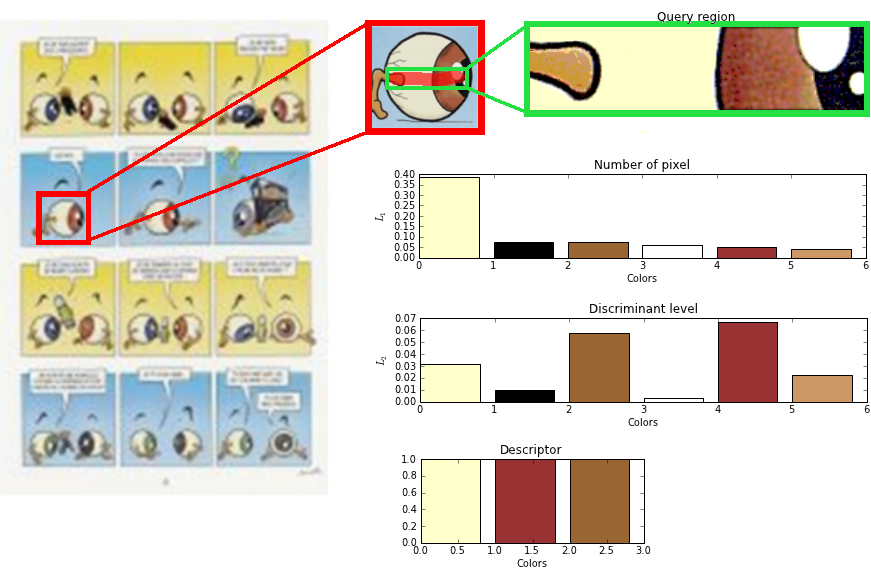
\includegraphics[width=0.9\textwidth]{description_sequence.png}
 	\caption[Comic character query description]{The left part represents a query example after the colour reduction process and its original image. Top-right part shows the colour histogram of the 6 first colours with the highest number of pixel in the query as a percentage from the total number of pixel in the query ($L_1$). Middle-right figure represents the corresponding discriminability level for each colour according the other pixel in the page. Bottom-right figure represents the corresponding query descriptor of $N=3$ colours.}
 	\label{fig:in:dominant_colour_hist_desc}
 \end{figure}
%%%%%%%%%%%%%%%%%%%%%%%%%%%%%%%%%%%%%%%%%%%%%%%%%%%


%------------------------------------------------------------------------
\subsection{Object retrieval}
Comics have a particular structure that allows different approaches for object retrieval. An interesting point is that a same instances of objects often appear in different panels and therefore several times in each page of the album.
%, which allow to searcat permits to think about searching other object occurrences.% from in the same image as the query and the others.

First, for a given page, we consider each colour value in the descriptor and compute the corresponding colour mask (Figure~\ref{fig:in:masks}). %Note, mathematical morphology may be used to remove isolated pixel noise (e.g. paper texture) in some cases.
Second we find the object position in each pages by using a sliding window approach at different window size and for each mask.
The window sizes are defined according to the user query size (maximum between the query width or height) which gives an information about the definition of the document $S=\{s_0,s_1,...,s_n\}$ in order to retrieve the object at different scales.
Each window position is computed with 50\% percent overlapping with its four neighbouring windows.

%%%%%%%%%%%%%%%%%%%%%%%%%%%%%%%%%%%%%%%%%%%%%%%%%%%
 \begin{figure}[!ht]  %trim=l b r t  width=0.5\textwidth,
   \centering
  \includegraphics[width=0.8\textwidth]{masks.png}
  \caption[Colour mask corresponding to five colour of the query descriptor]{Example of colour mask corresponding to the 5 first colours in the top histogram of Figure~\ref{fig:in:dominant_colour_hist_desc}.}
  \label{fig:in:masks}
 \end{figure}
%%%%%%%%%%%%%%%%%%%%%%%%%%%%%%%%%%%%%%%%%%%%%%%%%%%


We define the detection confidence $C_{w_i}$ according to the number of identical colours between the query descriptor $D$ and each sliding window positions $W=\{w_0,w_1,...,w_n\}$ (Equation.~\ref{eq:in:confidence_character_spotting}).
This is equal to the cardinality of the intersection between the two colour set $D \cap w_i$. The confidence is maximal when all the colours in the query descriptor are contained by the window (high probability of the object to be at this location).
The confidence $C_{w_i}$ is defined as follow:

\begin{equation}\label{eq:in:confidence_character_spotting}
   C_{w_i} = \frac{|D|}{|D \cap w_i|}\\
 \end{equation}
where $C_{w_i}$ is the confidence value for the region $w_i$, $|D|$ the cardinality of the colour set $D$ and $|D \cap w_i|$ the cardinality (number of element) of the intersection between $D$ and $w_i$ .

The confidence value is compared to a threshold value $T$ to decide whether or not the detection is correct. By using a multi-scale approach, a same region may be detected at different scales. In order to keep only the smallest region that include a minimal amount of background information, we compute the percentage of pixel $p$ which are of a colour from the descriptor for each detection region. 
A post processing step removes multiple object detections by keeping only the regions (windows) that are not overlapped by other regions with a higher $p$ value (best detected). See algorithm~\ref{al:in:retrieval} and Figure~\ref{fig:in:filtering}.

\begin{algorithm}
\caption{Object retrieval}
\label{al:in:retrieval}
\begin{algorithmic}
%\REQUIRE $n \geq 0 \vee x \neq 0$
%\ENSURE $y = x^n$
%\STATE $y \leftarrow 1$
%\State{compute $E_{ext}$ energy}
\STATE{//Detection}
\FOR{each $s$ in $S$}
  
  \FOR{each $w$ in $W$}
    
    \IF{$C(w) >= T$}
	\STATE add $w$ to the detected region list $R$
    \ENDIF  
  \ENDFOR
\ENDFOR

\STATE{}
\STATE{//Filtering}
\FOR{each $r$ in $R$}
    \IF{$r$ does not overlap better detected region}
	     \STATE $r$ is a candidate region
    \ENDIF
\ENDFOR
\end{algorithmic}
\end{algorithm}



%%%%%%%%%%%%%%%%%%%%%%%%%%%%%%%%%%%%%%%%%%%%%%%%%%%
 \begin{figure}[!ht]  %trim=l b r t  width=0.5\textwidth,
   \centering
  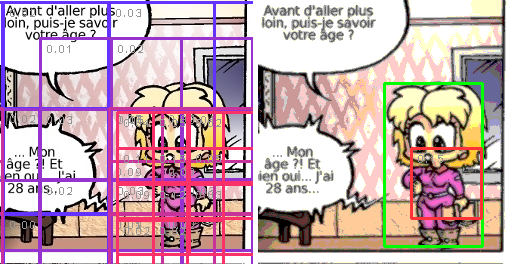
\includegraphics[trim= 0px 1px 0mm 0mm, clip,width=0.7\textwidth]{filtering.png}
  \caption[Multi-scale comic character spotting]{Multi-scale spotting example. The left image shows the detections at different scales, the colouration depends on to the $p$ value, blue to red for low to high. The right side image shows the remaining best detection after the filtering step. }
  \label{fig:in:filtering}
 \end{figure}
%%%%%%%%%%%%%%%%%%%%%%%%%%%%%%%%%%%%%%%%%%%%%%%%%%%


% subsection character_clustering (end)

\section{Conclusions}
\label{sec:in:conclusion}

In this chapter we have proposed independent extraction methods for panel, text, balloon and comics characters.

%PANEL
The panel extraction method is simple, fast and efficient for comics layout that have disconnected panels as the method relies on outermost contour analysis.
This method is experimented Section~\ref{sub:ex:panel_extraction_evaluation}.
%TEXT
The proposed approach for text extraction consists in an adapted bi-level segmentation followed by a filtering process of three steps based on contrast, topology and local similarities to classify the connected-components as graphics or text region.
A final text line level verification valid the textual content of the candidate regions using an OCR system.
The method does not requires previous knowledge about the image content unlike the sequential approach proposed Section~\ref{sec:se:panel_and_text} that is implicitly linked to the panel regions.
This method is experimented Section~\ref{sub:ex:text_extraction_recognition_evaluation}.

%BALLOON EXTRACTION, CLASSIFICATION AND TAIl
Independent balloon extraction and classification methods have been presented.
The balloon extractor relies on topological and spatial relations similarly to the text extraction method.
In fact, balloon and text extractions are often correlated in the literature as well because those regions are often associated to convey most of the textual information of comics.
As mentioned earlier, tail detection without previous balloon segmentation makes no sense because it is a specific region of the balloon contour.
This method is experimented Section~\ref{sub:ex:balloon_extraction_evaluation}.
%CHARACTERS
Unsupervised comic characters extraction is a real challenge, here we proposed a user-defined query-based approach but it can be replaced by a comic characters region of interest, automatically computed from surrounding information (context) (Section~\ref{sec:se:tail_to_character}).
%GENERAL
In each extraction process, we strive to produce indicators of confidence, conscious that it could be useful for a higher level processing system such as that presented in the next chapter.

Next chapter is going to present a high level approach for understanding the image content and its semantic.
We will propose a model for both comic book's and image processing domains knowledge for information consistency analysis and relation inferences between all the extracted elements such as the reading order, the type of text (e.g. spoken, onomatopoeic, illustrative) and the positions of the speaking characters.

% This approach is based on a expert system coupled with an inference engine.

%In this chapter we have proposed a graph based approach for symbol spotting in graphical documents. We represent the documents with graphs where the critical points detected in the vectorized graphical documents are considered as the nodes and the lines joining them are considered as the edges. The document database is represented by the unification of the serialized substructures of graphs. Here the graph substructures are the acyclic graph paths between each pair of connected nodes. The factorized substructures are the one-dimensional (sub)graphs which give efficiency in terms of computation and since they provide a unified representation over the database, the computation is substantially reduced. Moreover, the paths give adaptation to some structural errors in documents with a certain degree of tolerance. We organize the graph paths in hash tables using the LSH technique, this helps to retrieve symbols in real time. We have tested the method on different datasets of various kinds of document images and the results are quite encouraging.

%In the next chapter we are going to propose a subgraph matching algorithm based on tensor product graph (TPG) (see \sect{sec:gm:pg} for details). Continuous optimization is a very popular approach in (sub)graph matching but it mostly works with pairwise measurements. But often pairwise quantifications are not reliable, to remove this problem in \ch{chap:pg} we propose walk based propagation of pairwise similarities to obtain contextual information incorporated in the higher order similarity measures. Then we formulate the subgraph matching problem as a node, edge selection problem in TPG. Also in \ch{chap:pg}, a \emph{dual edge graph} representation is proposed which achieves spatial relationship between the graph paths which was absent in this chapter.